\documentclass[pre,aps,floatfix,10pt,superscriptaddress, notitlepage,preprint]{revtex4-1}
\pdfoutput=1
\usepackage[english]{babel}
\usepackage[T1]{fontenc}
\usepackage[latin9]{inputenc}
\usepackage{amsmath,amssymb}
\usepackage[svgnames]{xcolor}
\usepackage{graphicx}
\usepackage{acro}
\usepackage{subfig}
\usepackage{caption}
\graphicspath{{figures/}}

\captionsetup[figure]{justification=raggedright}

\newcommand{\set}[1]{\ensuremath{\mathcal{#1}}}

\DeclareAcronym{pdf}{
	short=PDF,
	long=Probability Density Function,
}
\DeclareAcronym{iid}{
	short=i.i.d.,
	long=Independent Identically Distributed
}
\DeclareAcronym{ou}{
	short=OU,
	long=Ornstein-Uhlenbeck,
}
\DeclareAcronym{gktl}{
	short=GKTL,
	long=Giardina-Kurchan-Tailleur-Lecomte,
}
\DeclareAcronym{ams}{
	short=AMS,
	long=Adaptive Multilevel Splitting,
}
\DeclareAcronym{tams}{
	short=TAMS,
	long=Trajectory Adaptive Multilevel Splitting,
}
\DeclareAcronym{scgf}{
	short=SCGF,
	long=Scaled Cumulant Generating Function,
}
\DeclareAcronym{lbm}{
	short=LBM,
	long=Lattice Boltzmann Method,
}
\DeclareAcronym{lbe}{
	short=LBE,
	long=Lattice Boltzmann Equation,
}
\DeclareAcronym{lgca}{
	short=LGCA,
	long=Lattice Gas Cellular Automata,
}
\DeclareAcronym{lbgk}{
	short=LBGK,
	long=Lattice Bhatnagar-Gross-Krook
}
\DeclareAcronym{OU}{
	short=O-U,
	long=Ornstein--Ulhenbeck
}
\DeclareAcronym{dns}{
	short=DNS,
	long=Direct Numerical Simulation,
}
\DeclareAcronym{md}{
	short=MD,
	long=Molecular Dynamics,
}
\DeclareAcronym{cfd}{
	short=CFD,
	long=Computational Fluid Dynamics,
}


\newcommand{\EL}[1]{{\color{red}{#1}}}
\newcommand{\TL}[1]{{\color{green}{#1}}}

\begin{document}
	
\title{Rare-event sampling applied to the simulation of extreme mechanical efforts exerted by a turbulent flow on a bluff body}
	
\author{Thibault Lestang}
\email{thibault.lestang@ens-lyon.fr}
\affiliation{Univ Lyon, ENS de Lyon, Univ Claude Bernard de Lyon, CNRS, Laboratoire de Physique, F-69342 Lyon, France}
\affiliation{Univ Lyon, Ecole Centrale de Lyon, Univ Claude Bernard de Lyon, INSA de Lyon, CNRS, Laboratoire de M\'ecanique des Fluides et d'Acoustique, F-69134 Ecully cedex, France}
\author{Freddy Bouchet}
\email{freddy.bouchet@ens-lyon.fr}
\affiliation{Univ Lyon, ENS de Lyon, Univ Claude Bernard de Lyon, CNRS, Laboratoire de Physique, F-69342 Lyon, France}
\author{Emmanuel L�v�que}
\email{emmanuel.leveque@ec-lyon.fr}
\affiliation{Univ Lyon, Ecole Centrale de Lyon, Univ Claude Bernard de Lyon, INSA de Lyon, CNRS, Laboratoire de M\'ecanique des Fluides et d'Acoustique, F-69134 Ecully cedex, France}
	
	
	
\begin{abstract}
	\EL{ ABSTRACT TO BE REVIEWED}
This study evaluates the relevance of  rare-event sampling to optimize the numerical simulation of extreme mechanical efforts exerted by a turbulent flow impinging onto a bluff body. The main idea is here to replace a long simulation by a set of much shorter simulations (running in parallel) with dynamics that are replicated or abandoned in order to sample large-amplitude events more frequently. 
%
Such technique has already proved its efficiency for simulating extreme events in {...} with significant run-time savings.
Application to fluid-structure interaction problems remains mainly open. 
%
The drag experienced by a squared obstacle placed in a turbulent flow (in two dimensions) is taken as a representative case study to investigate the performance of two major sampling algorithms, namely {...} 
Practical evidence is given that these algorithms allow for the correct sampling of rare large-amplitude drag events and the estimation of return times with a reduced computational effort. However, {limitations and pitfalls}. 
% Importantly, such techniques also provide direct access to the flow scenario yielding extreme events. In the present case, it is found that {<blocking effect>}.
\end{abstract}
	
\maketitle
	
\section{Introduction}
	
% general comments on physical problem %
%
Turbulent flows are important in a variety of natural phenomena, industrial and civil applications with the characteristic feature to spontaneously develop intense and sporadic motions associated with extreme internal forces \cite{lesieur_book,donzis_sreenivasan_2010,Yeung}. ``Extreme'' refers here to fluctuations that can deviate from mean value by ${\cal{O}}(10)$ standard deviations. In engineering, the nature of such extreme dynamical events and their statistics are of crucial interest to predict excessive mechanical efforts. Such anomalous efforts can threaten the structural integrity of embedded structures.
%
From the viewpoint of (chaotic) dynamical systems, turbulence in fluids has to do with non-linearity and strong departure from statistical equilibrium \cite{KRAICHNAN}. The use of perturbative methods in identifying resonant interactions (among degrees of freedom) possibly responsible for extreme fluctuations is not successful. Therefore, simulation offers a practical means to gain physical insight into these events, quantify their intensity and estimate their frequency of occurrence. Nevertheless, this requires very long simulation since these events are also very rare. It is here our motivation to evaluate the practicality and efficiency of rare-event sampling techniques to alleviate this prohibitive computational cost. 
%	
	
% general def on rare-event sampling %
%
Rare-event sampling is an umbrella term for numerical methods intended to sample preferentially regions of the phase space which would otherwise be rarely visited  through brute-force simulation.
%
	
%
% next two paragraphs may be too technical -- Find a way to summarize them in a few sentences accessible to a broad audience in fluid mechanics? Notion of action will be vague for many readers
%
% this paragraph would certainly need to be reshaped!
%
In fluid turbulence, rare-event sampling has been approached mainly from simplified dynamics such as the one-dimensional Burgers' equation with a stochastic forcing \cite{bec_burgers_2007}. In that case, dynamics may be accounted for through an action that can be identified as analogous to a Gibbs measure for a system at equilibrium. This latter can be sampled by using a Markov chain Monte-Carlo  algorithm \cite{duben_monte_2008,mesterhazy_anomalous_2011,mesterhazy_lattice_2013} that provides a framework for rare-event sampling.
%
An alternative approach is based on \emph{instanton} \cite{grafke_instanton_2015}. For stochastically driven systems in the limit of weak noise, it can be proved that the probability of extreme events is dominated by the minima of the action \cite{freidlin2013random} -- the trajectories that achieve such minima being referred to as instantons \cite{gurarie_instantons_1996}. Therefore, suitable numerical schemes can  be used to minimize the action and evaluate instantons as well as the related probabilities of rare events \cite{chernykh_large_2001,grafke_instanton_2013,grafke_relevance_2015,grigorio_instantons_2017}.
%
An obvious drawback of the aforementioned approaches is their limitation to stochastically driven dynamics which, in addition, must be simple enough so that an action may be derived and sampled, or minimized. 
%
%
%Whilst Burgers' turbulence provides an interesting model framework for the investigation of the properties of small scale turbulence, it is of little relevance to more realistic situations, such as industrial or environmental flows.
%
In this paper, a more general approach is investigated. It relies on sampling algorithms connected to the simulation of the actual dynamics itself, \textit{i.e.} applying directly to the trajectories in the dynamic space.
% dedicated to dynamical systems for which an action cannot be easily derived or minimized,
%    
%
Even though such ideas trace back to the early 1950's, they have received ever-growing interest over the last 20 years with successful applications in various domains such as chemistry \cite{van_erp_elaborating_2005,escobedo_transition_2009,teo_adaptive_2016}, biophysics \cite{huber_weighted-ensemble_1996,zuckerman2017weighted,bolhuis2005kinetic}, nuclear physics \cite{louvin2017}, nonlinear dynamical systems \cite{tailleur_probing_2007} or communication networks simulation \cite{villen-altamirano_restart:_1994}.
%
% already mentioned in the beginning? This sentence is misleading.
%
%However, a large body of algorithms are limited to systems at equilibrium, for which the stationary measure can be sampled by means of Monte Carlo methods. 
%
An original contribution of the present study is certainly the application of rare-event sampling algorithms in the context of far-from-equilibrium dynamics with an irreducible very large number of degrees of freedom. 
Let us remark that most of previous successful applications involve dynamical systems at statistical equilibrium and low-dimensional attractors. \EL{is it TRUE?}
% 
Two different algorithms suitable for out-of-equilibrium dynamics are considered and compared. Namely, the Adaptive Multilevel Splitting algorithm and the Giardina-Kurchan-Tailleur-Lecomte algorithm.
%
	
The Adaptive Multilevel Splitting (AMS) algorithm \cite{cerou_adaptive_2007} inherits from old ideas about splitting approaches \cite{KahnHarris1951,glasserman_look_1998,glasserman_multilevel_1999} -- a detailed description will be given later.  
In recent years, this algorithm has allowed for the computation of rare events in problems involving a large number of degrees of freedom such as molecular dynamics simulations \cite{aristoff_adaptive_2015,teo_adaptive_2016}, the computation of rare trajectories in the Allen-Cahn equations \cite{rolland_computing_2016} or rare events of re-laminarization in a stochastic model of wall-turbulence \cite{rolland_extremely_2018}.

Over the last decade, the main theoretical framework for the study of rare events (in statistical physics) has been the theory of large deviations \cite{touchette_large_2009}.
Alongside, numerical methods have been developed to sample rare events \cite{moral_feynman-kac_2004}. 
Among them, the \ac{gktl} algorithm \cite{giardina_direct_2006} is particularly suited for (chaotic) dynamical systems \cite{giardina_simulating_2011,Laffargue_2013}.
%
Recently, \ac{gktl} has allowed to successfully perform the numerical simulation of extreme heat waves in a simplified modeling of the atmosphere \cite{ragone_computation_2018}. 
This achievement represents a significant leap in the applicability of rare-event sampling to complex dynamical systems. Along the same line, rare-event sampling algorithms are here pushed aside traditional applications by considering fluid-structure interaction in a turbulent flow. 
	

	
\section{Description of the numerical case study}
\label{sec:test_flow}
	
\begin{figure}
\centering
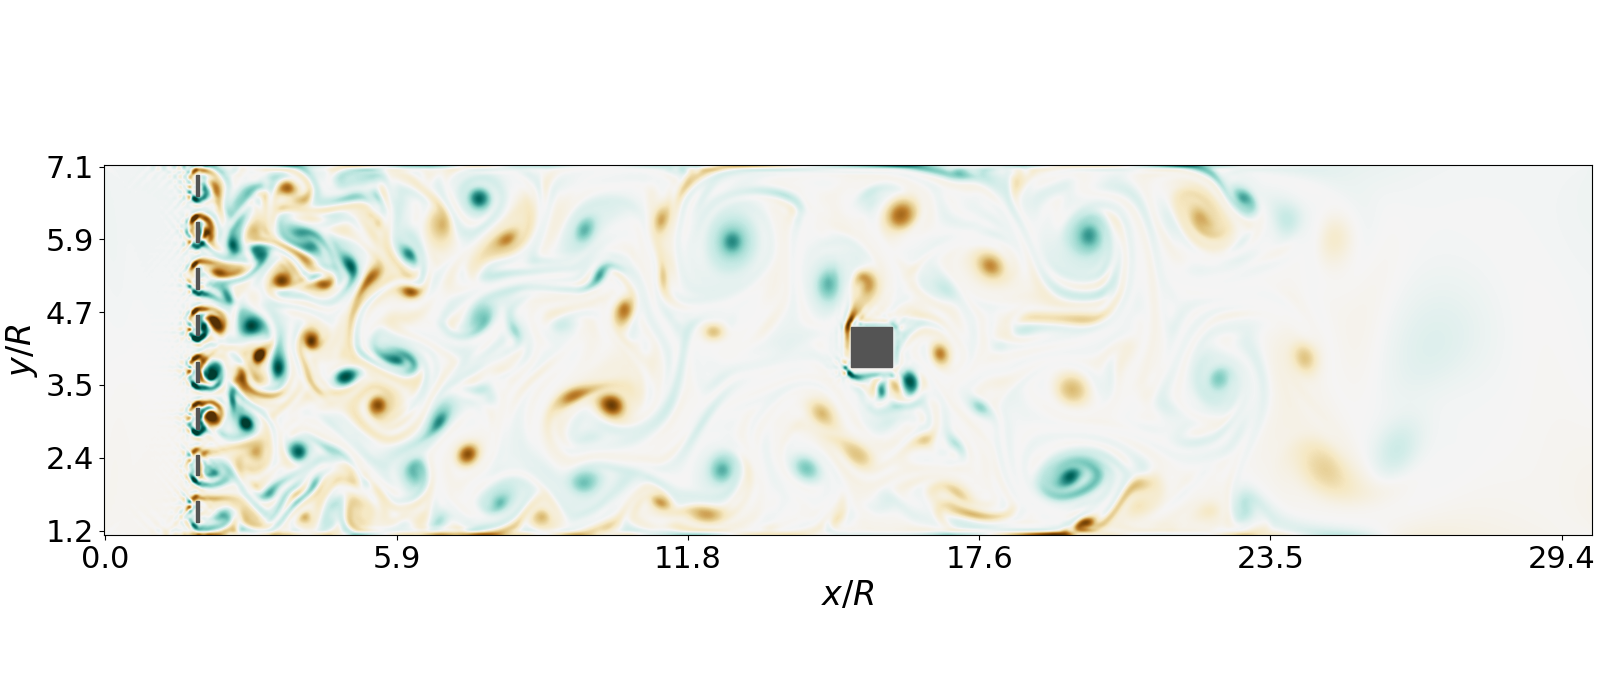
\includegraphics[width=\linewidth]{illustr_ecoulement/illustr_ecoulement}
\caption{Our case study is a grid-generated turbulent flow impinging onto a fixed squared obstacle (of size $R$) located at the center of a channel in two dimensions. The flow is artificially damped near the end of the channel. In the developed flow, turbulent eddies have typically the size of the square, which results in strong fluctuations of mechanical efforts acting on the square. The vorticity is displayed with an arbitrary color map from blue (negative values) to red (positive values).}
\label{fig:illustr_ecoulement}
\end{figure}
	
% introduce the flow 
%
The drag exerted by a grid-generated turbulent flow onto a fixed squared obstacle is considered as a representative case study (see Fig.~\ref{fig:illustr_ecoulement}). 
% why this flow?
%
Although real-world applications would eventually imply three-dimensional dynamics, a simplified two-dimensional setting has been chosen here to reduce the computational cost and allow for a systematic study. 
% 
We believe that this system embeds the characteristic features that makes the application of rare-event algorithms both relevant and challenging for fluid-structure-interaction problems. 
%Namely, spatio-temporal chaos and the emergence of large-amplitude mechanical efforts on the structure.
%
% rapid description of the flow
Turbulent eddies generated in the near-wake of the grid are carried downstream. They interact with each other and grow in size as expected in two-dimensional turbulence. 
The dimension of the grid is such that the size of the eddies that eventually hit the square is comparable to the size of this latter, which results in strong fluctuations of the drag acting on the square. 
%
%Finally, the obstacle does not deform or move either. 
%
%Through this simplified setting, our motivation is primarily to evaluate the operability of sampling techniques to capture extreme events with a significant run-time savings.  
%


% lattice Boltzmann method 
%
The flow dynamics is integrated by the lattice Boltzmann (LB) method in our numerical simulations. 
While traditional methods in \emph{computational fluid dynamics} rely on a discretization of the Navier-Stokes equations, the LB method considers the fluid at a mesoscopic level. Capturing the dynamics of collections of fluid particles distributed on a lattice is here preferred to solving non-linear PDEs. 
%This seems crazy, however, most details at the mesoscopic level play actually no role at the macroscopic level. Therefore, the LB algorithm may be viewed as a minimal kinetic scheme compliant to the fluid dynamics at the macroscopic level.
Further details are given in Appendix and references therein.
In our situation, the LB method has been chosen principally for its outstanding computational efficiency. 


% geometry
%
The simulated flow develops in a long plane channel of dimension $512 \times 128$ mesh points. The squared obstacle has size $R=16$ (in mesh unit) and is located at the center of the channel. The spacing and bar height of the entrance grid are both equal to $R/2$ (see Fig.~\ref{fig:illustr_ecoulement}). 
% boundary conditions
%
No-slip boundary conditions are enforced on top and bottom walls of the channel and on the surface of the obstacle by using an halfway bounce-back procedure \cite{lbm_book}.  
%
Upstream the grid, a constant parabolic velocity profile and a constant mass density (equal to unity) are imposed as inlet condition. 
The centerline velocity is $0.05$ in lattice unit, \textit{i.e.} normalized by $\Delta x/\Delta t$ with $\Delta x$ and $\Delta t$ referring to the lattice resolution and the time-step respectively. The distributions are imposed at equilibrium (see Appendix). 
In the bulk, the viscosity is adjusted to generate grid turbulence with Reynolds number $\mathrm{Re_{grid}}=1200$. The reference Mach number is equal to $0.06$ in agreement with the assumption of weak compressibility of the LB method. 
Near the end of the channel, the flow is progressively damped within a \textit{sponge layer} where the viscosity is artificially enhanced. Finally, the oulet boundary condition relies on a second-order extrapolation of the velocity and mass density. The extrapolated distributions are evaluated through a regularization procedure relying on a finite difference estimation of the local stress tensor, as introduced in \cite{latt2008straight}. 

	
\subsection{The drag force}
\label{sec:drag_force}
	
\begin{figure}
	\centering
	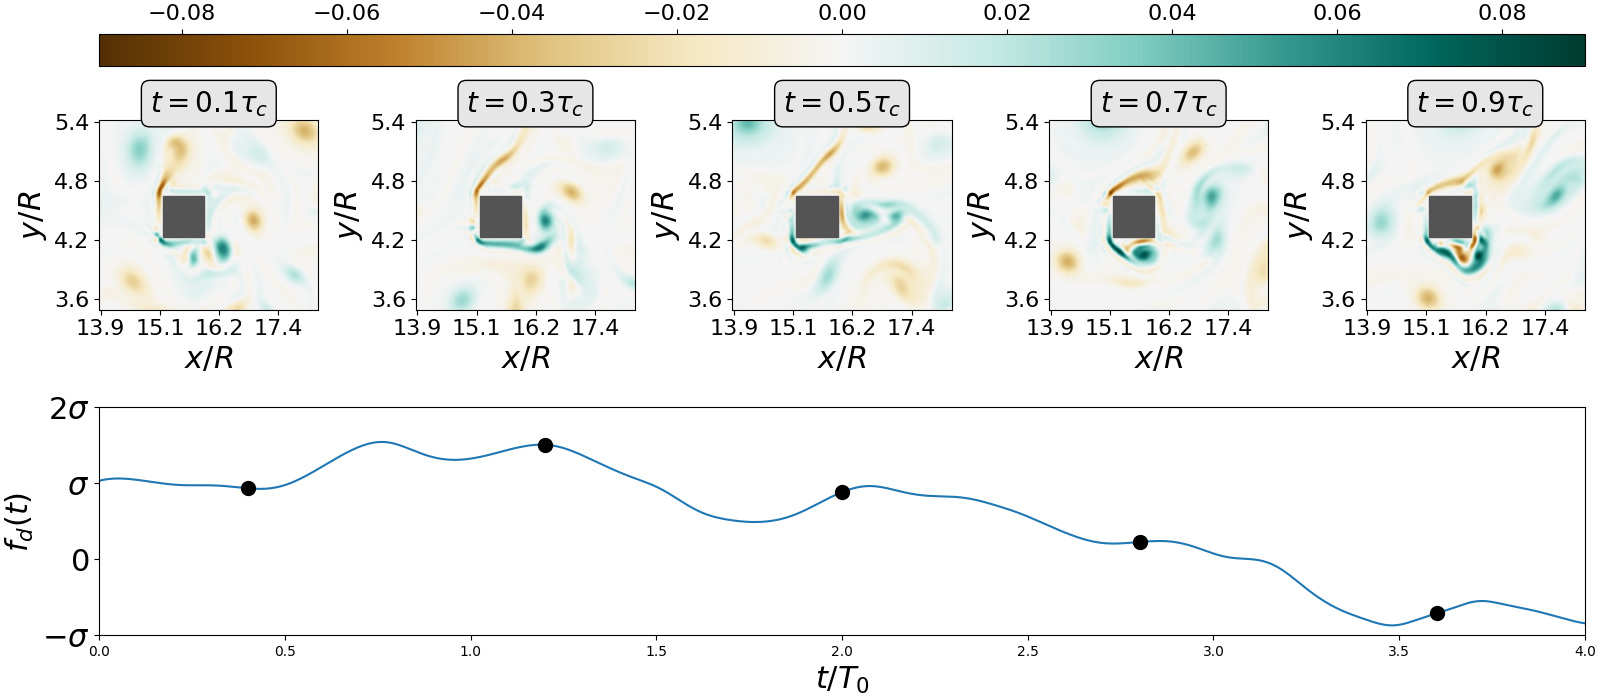
\includegraphics[width=\linewidth]{ecoulement_typique/ecoulement_typique.png}
	\caption{Snapshots of the vorticity related to typical drag fluctuations (within one standard deviation) over a time interval of length $\tau_c \simeq 4\tau_0$; $\tau_c$ will be identified later as the correlation time of the drag signal.
	The vorticity is given in lattice units. \EL{THE COLORMAP IS REVERSED IN THE WHOLE PAPER: BLUE SHOULD BE NEGATIVE AND RED POSITIVE}}
	\label{fig:typical_vorticity}
\end{figure}


% drag signal
%
The incoming turbulent flow exerts fluctuating mechanical efforts onto the squared obstacle. The \textit{drag} is defined as the resulting force in the streamwise $x$-direction and expresses formally as 
\begin{equation}
\label{eq:drag_definition}
f_d(t) = \int_{\mathcal{S}} \boldsymbol{\tau}_{x \beta}(\mathbf{x},t) ~ \mathrm{d}{\mathcal{S}}_\beta(\mathbf{x})  
\end{equation}
where $\mathcal{S}$ is the surface of the obstacle and $\boldsymbol{\tau}$ denotes the stress tensor (see Appendix). 
Here, the viscous stress makes a negligible contribution to the drag, which therefore results mostly from pressure forces.
% which are closely related to the distribution of velocity gradients in the vicinity of the obstacle (in the nearly-incompressible limit). 
%
Since the pressure on the top and bottom sides of the square applies in the normal direction, they do not contribute to the drag. 
As a consequence, the drag can be expressed as the pressure difference 
\begin{equation}
\label{eq:drag_approx}
f_d(t) = p_{fb}(t) - p_{base}(t)
\end{equation}
between the pressure integrated over the forebody, $p_{fb}(t)$, and the base of the obstacle, $p_{base}(t)$.
	
% Definition of turnover time
%
The typical timescale (turnover time) of drag fluctuations may be estimated from dimensional analysis as
\begin{equation}
\label{eq:turnover_time}
\tau_0 = \frac{R}{U}
\end{equation}
where $R$ is the size of the square and $U$ the averaged velocity. 
The viscosity is here discarded since viscous stress is negligible as compared to pressure forces.
%
% typical fluctuation of the drag
%
Fig.~\ref{fig:typical_vorticity} displays the typical evolution of the vorticity field around the obstacle over a few turnover times. It is observed that, typically, some vorticity is generated near the front part of the obstacle, rapidly detach from it and is advected downstream by the flow.
Therefore, the \textit{base pressure} varies much less than the \textit{forebody pressure} and typical drag fluctuations  result mostly from the variation of the pressure at the front of the obstacle.
In section~\ref{sec:direct_sampling}, we shall highlight that the situation leading to  {extreme} fluctuations of the drag is different.
%In particular, extreme fluctuations mainly result from large variations of the base pressure, whereas forebody pressure variations play a lesser role.

\subsection{The drag as a random process: Probability Density Function, correlation in time}
\label{sec:pdfs}

\begin{figure}
	\centering
	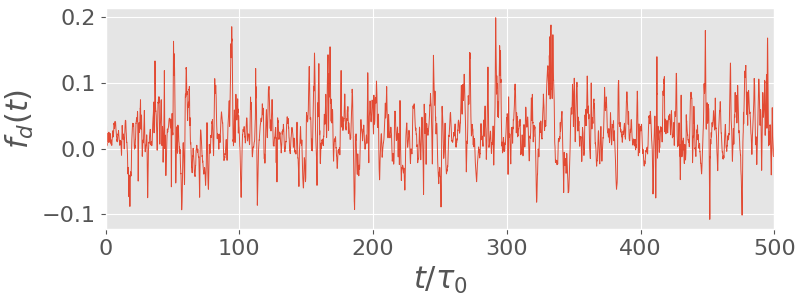
\includegraphics[width=0.7\linewidth]{typical_drag_signal/typical_drag_signal.png}
	\caption{Temporal evolution of the drag (in lattice units) acting on the square under the action of the impinging turbulent flow. The time is normalized by the turnover time related the mean-flow velocity and the size of the obstacle, \emph{i.e.} $\tau_0=R/U$.}
	\label{fig:typical_drag_signal}
\end{figure}


% drag signal
%
Fig.~\ref{fig:typical_drag_signal} shows the time signal of the drag acting on the square, $f_d(t)$, over five hundred turnover times. The signal appears unpredictable in details and exhibits repeated bursts of high amplitude that deviate significantly from the averaged value.
It is therefore natural to consider the drag as a random process.


\begin{figure}
  \centering
    \subfloat[\ac{pdf} of (zero-mean) drag fluctuations]
    {\label{fig:pdf_drag_a}
    	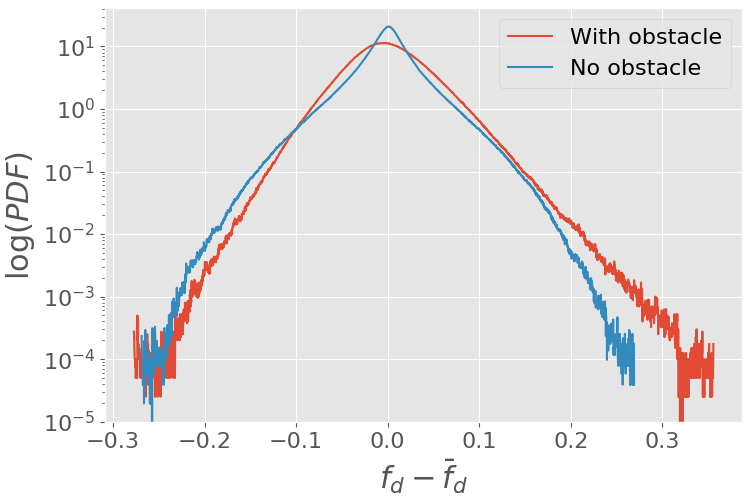
\includegraphics[width=.45\linewidth]{./PDF_drag/PDF_drag.png}}
    \subfloat[Autocorrelation of drag fluctuations]
    {\label{fig:pdf_drag_b}
    	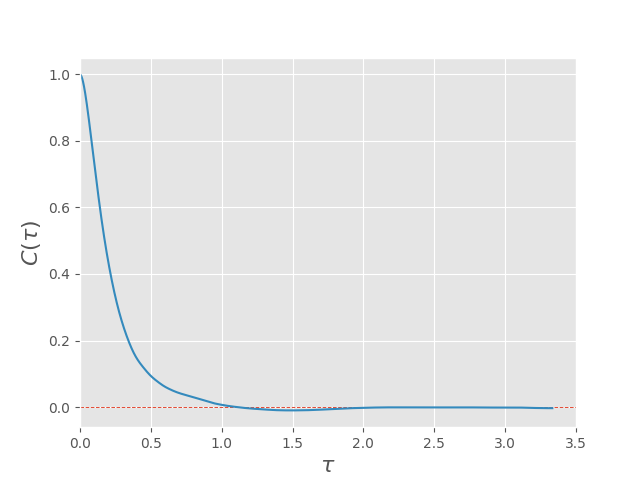
\includegraphics[width=.45\linewidth]{./autocorr_drag/autocorr_drag.png}}  
      \caption{\textbf{(a)} \ac{pdf} of (zero-mean) drag fluctuations $\tilde f_d \equiv f_d - \bar{f_d}$ where $\bar{f_d}$ denotes the time-averaged value. The drag is evaluated both in the presence (red) and in the absence (blue) of the obstacle. %Note that the amplitudes have not been normalized.
  \textbf{(b)} Autocorrelation function of the drag defined as $C(\tau) = \overline{ \tilde f_d(t+\tau)\tilde f_d(t)} ~/~ \overline{{\tilde f_d}^2}$. The correlation time $\tau_c$ is given by $C(\tau_c)=0$.
  %$\tau_c$ may therefore be considered as the correlation time of the drag signal.
}
  \label{fig:pdf_drag}
\end{figure}

% drag statistics
% PDF and correlation time
%
Drag fluctuations have been recorder during a simulation of duration $T_{tot} = 4 \times 10^6~\tau_0$. This very long simulation will be referred to as the \textit{control run} in the remainder. It has been made possible by the relative simplicity of the investigated two-dimensional flow and the computational efficiency of the Lattice Boltzmann method. 
%The related execution time is about a few weeks (wall-clock time).
The \ac{pdf} of the drag fluctuations is displayed in Fig.~\ref{fig:pdf_drag_a}.
It deviates from a normal law and exhibits an exponential tail for large positive values, \textit{i.e.}  ${\mathbb{P}}(\tilde f_d) \propto e^{-\lambda \tilde f_d}$.
%
Fig.~\ref{fig:pdf_drag_a} also shows the \ac{pdf} of drag fluctuations acting on a control surface corresponding the periphery of the obstacle but in the absence of the obstacle. 
%
In that latter case, the \ac{pdf} is quasi-symmetric and does not display exponential tails. This suggests that the asymmetry of the \ac{pdf} and the positive exponential tail are closely related to the no-slip condition on the obstacle.
%
%
Lastly, the autocorrelation function of the drag $C(\tau)$ is shown in Fig.~\ref{fig:pdf_drag_b}. It is found that drag fluctuations are correlated over a time interval $\tau_c \simeq 4\tau_0$ for which $C(\tau_c)=0$. Therefore, the drag looses its memory  over a time scale corresponding to the sweeping of a few eddies past the obstacle.
%
This observation will have important consequences for the application of rare-event algorithms, as will be discussed in section~\ref{sec:rare_events_algorithms}.
%
In the following, $\tau_c$ will be referred to as the \textit{correlation time} of the drag. The ratio $\tau_0 / \tau_c$ may be viewed as a {Strouhal number}; $St=0.25$ is consistent with commonly observed values for flows past blunt structures.


\section{Extreme fluctuations of the drag by means of direct sampling}
\label{sec:direct_sampling}


\begin{figure}
	\centering
	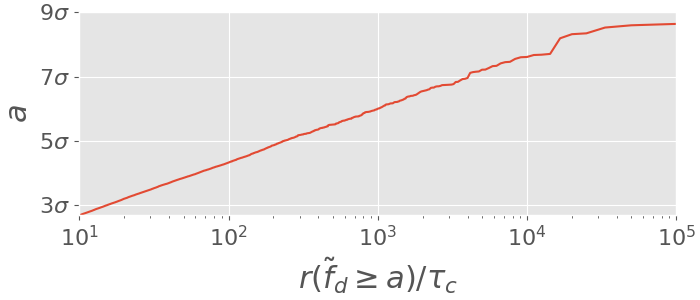
\includegraphics[width=.6\linewidth]{return_time/return_time.png}
	\caption{Amplitude of drag fluctuation (in standard-deviation unit) as a function the corresponding return time. The return time $r(a)$ is defined as the typical period of occurrence of a fluctuation of amplitude $a$.}
	\label{fig:return_time_instant}
\end{figure}

% return time given from direct sampling
%
At first, the phenomenology of extreme fluctuations of the drag is investigated by means of \textit{direct sampling} of the control run. This brute-force approach is here used as opposed to optimized approaches involving rare-events algorithms discussed in section~\ref{sec:rare_events_algorithms}. The direct approach will provide a trustworthy baseline for the validation of rare-events algorithms. 

How rare is a fluctuation $f_d \geq a$ can be quantified by its so-called \textit{return time} $r(a)$. This latter is defined as the average time between two consecutive occurrences of events of amplitudes $f_d \geq a$\TL{, as illustrated in figure~\ref{fig:illustrate_return_time}.}
\begin{figure}
  \centering
  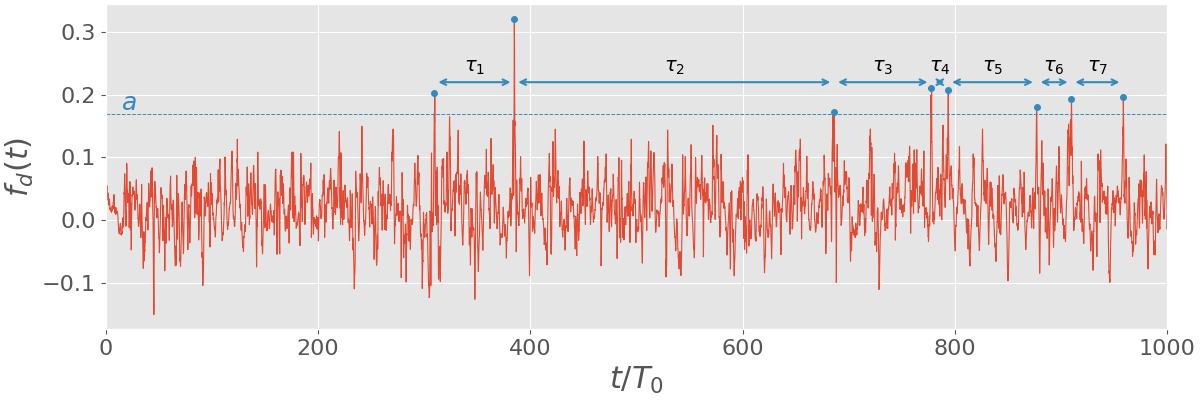
\includegraphics[width=\linewidth]{illustrate_return_time/illustrate_return_time}
  \caption{\label{fig:illustrate_return_time} \TL{The \textit{return time} $r(a)$ of a fluctuation $f_d \geq a$ is defined as the average waiting time between the occurence of the event: $r(a) = \mathbb{E}[\tau]$. Note that we assume $r(a) >> \tau_0$, and therefore consider that such events are points in time.}}
\end{figure}
Extreme drag fluctuations are \textit{rare events} in the sense that the return time is much larger than the correlation time: $r(a) \gg \tau_c$.
In that case, the occurrence of such events follows a Poisson process \cite{lestang_computing_2018} and
\begin{equation}
  \label{eq:return_time}
  r(a) \underset{a\to\infty}{\propto} \frac{1}{\mathbb{P}(f_d\geq a)} \propto e^{\lambda a}
\end{equation}
where $\lambda$ is the rate describing the positive tail of the \ac{pdf} of the drag (shown in Fig.~\ref{fig:pdf_drag}).
%
Fig.~\ref{fig:return_time_instant} illustrates the evolution of the return time $r(a)$ with the amplitude of fluctuation $a$ computed from the \textit{direct sampling} of the drag signal $f_d(t)$ \cite{lestang_computing_2018}. It is found that the return time indeed diverges  exponentially with the amplitude of fluctuation. Let us also remark that under-sampling effects explain the deviation from the exponential law at the largest amplitudes.
% typically for $a \gtrsim 8 \sigma$ with $\sigma$ being the standard deviation. 



\subsection{Extracting extreme drag fluctuations from a very long timeseries}
\label{sec:extreme_extraction}

% intro
%
We have extracted  the fluctuations of the drag with a return time $r(a)$ greater than  $10^4~\tau_c$ from the control time-series $\{f_d(t)\}_{0 \leq t \leq T_{tot}}$. This set will be considered as representative of \emph{extreme events} in the upcoming study. The choice of this particular threshold has been driven by the need to collect enough large-amplitude events and possibly identify generic features.
%
According to Fig.~\ref{fig:return_time_instant}, the related amplitude $a$ is found equal to $7.6~\sigma$ with $\sigma$ being the standard deviation. Precisely, 104 independent excursions \EL{excursion, terminologie correcte?} with $f_d(t) \geq 7.6~\sigma$ have been identified. For convenience, each excursion will be characterized in the following by its maximal value $f_d^{\star}$ and the time $t^{\star}$ at which this maximum is reached.
%
The phenomenology of extreme drag fluctuations will be examined on the basis of this set of events.


\subsection{Instantaneous drag}
\label{sec:instantaneous_drag}

\subsubsection{Contribution of forebody and base pressure fluctuations to the overall drag fluctuation}
\label{sec:forebody_and_base_contribution}

\begin{figure}
	\centering
	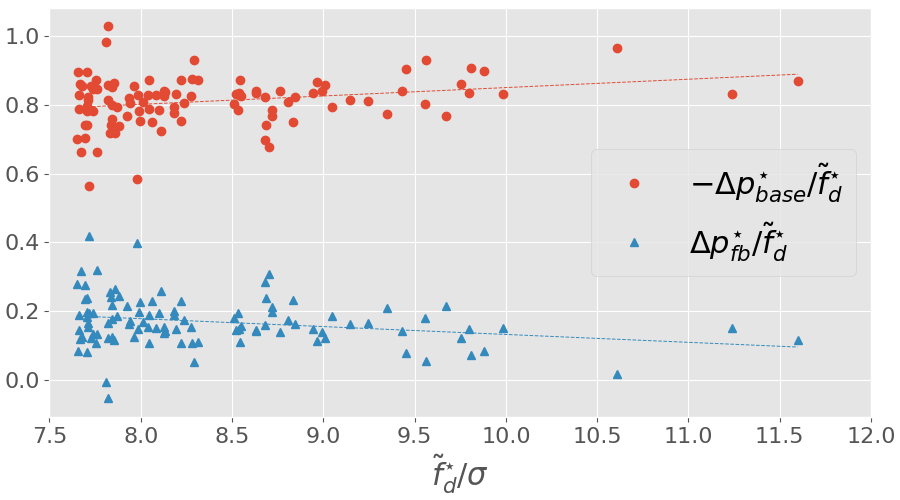
\includegraphics[width=.8\linewidth]{pressure_ratio/pressure_ratio.png}
	\caption{\label{fig:pressure_ratio} Relative contributions of the forebody and base pressure variations to extreme amplitudes of the drag. An extreme event corresponds to an amplitude $\tilde f^{\star}_d$ and a unique pair  ($\tilde{p}^{\star}_{base}$,~$\tilde{p}^{\star}_{fb}$).
	As the amplitude of the drag increases, the relative variation of the base pressure also increases. \EL{in Figure, $\tilde{p}_{fb}^{\star}/\tilde{f}_d^{\star}$ and $-\tilde{p}_{base}^{\star}/\tilde{f}_d^{\star}$} }
\end{figure}

% teasing
%
In section~\ref{sec:test_flow}, it has been pointed out that typical drag fluctuations  originate mostly from the variation of the forebody pressure, \textit{i.e.} from the upstream turbulent flow. We shall see that the situation is different in the case of {extreme} drag fluctuations. 

% relative contribution of forebody and base pressure
%
Let $(t^{\star}, f_d^{\star})$ refer to an extreme drag event.
The (zero-mean) fluctuation $\tilde{f}_d^{\star} = f_d^{\star} - \overline{f_d}$ can be  decomposed into 
\begin{equation}
  \tilde{f}_d^{\star} = \tilde{p}_{fb}^{\star} - \tilde{p}_{base}^{\star}
\end{equation}
where $\tilde{p}_{fb}^{\star}$ and $\tilde{p}_{base}^{\star}$ denote the variations of the forebody pressure and base pressure, respectively.
%
Fig.~\ref{fig:pressure_ratio} displays the relative contributions
$\tilde{p}_{fb}^{\star}/\tilde{f}_d^{\star}$ and $-\tilde{p}_{base}^{\star}/\tilde{f}_d^{\star}$ to the overall drag fluctuation $\tilde f_d^{\star}$.
\EL{please confirm signs! I have added a minus sign: $-\tilde{p}_{base}^{\star}$}  
%
It is found that the base pressure variation contributes typically $80\%$ to the overall drag fluctuation. Therefore, extreme amplitude of the drag are dominated by the variation of the pressure in the vicinity of the base of the obstacle, \emph{i.e.} downstream the obstacle.
Furthermore, Fig.~\ref{fig:pressure_ratio} suggests that the larger the fluctuation, the more important is the relative contribution of the base pressure. 
%relatively to the forebody pressure.



\subsubsection{Fluid dynamics related to extreme drag fluctuations}
\label{sec:dynamical_aspects}

\begin{figure}
	\centering
	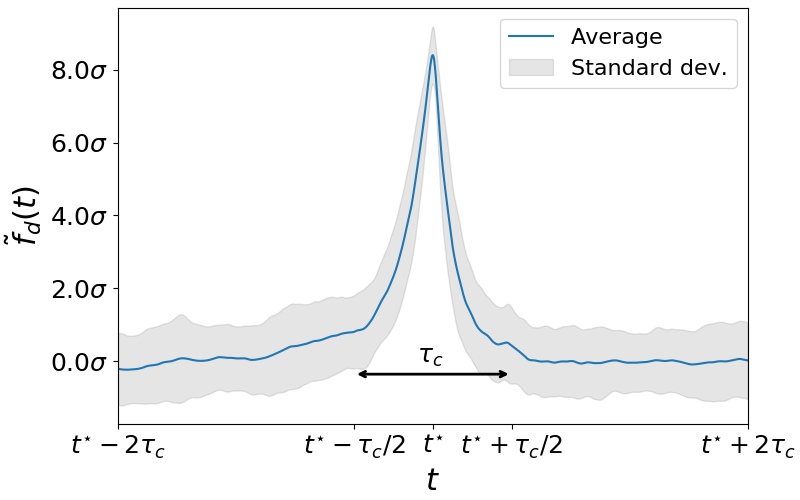
\includegraphics[width=.7\linewidth]{timeseries_extremes/timeseries_extremes.png}
	\caption{\label{fig:timeseries_extremes} Ensemble average of drag signals centered around extreme fluctuations occurring  at $t=t^{\star}$. The blue line shows the mean profile whereas the shaded area indicates variations (around the mean profile) within one standard deviation. Extreme drag events exhibit a typical lifetime of one correlation time $\tau_c$. The profile is slightly skewed indicating that the step up is slower than the return to typical values. \EL{ $\tilde f_d$ rather than $f_d$ in figure?}}
\end{figure}

% mean profile around burst
%
The focus is now on the flow scenarii that yield extreme values of the drag. 
Fig.~\ref{fig:timeseries_extremes} displays the mean profile (in time) of the drag signal around extreme events. A peaked profile is observed with a width corresponding roughly to one correlation time $\tau_c$. This implies that the duration of extreme events corresponds typically to the sweeping time of the flow past the obstacle. 
%Starting from typical values, extreme drags are typically reached in less than a correlation time. 
Interestingly, the profile is also slightly skewed indicating that the step up of the drag  is slower than the return to typical values past the peak value.
%Moreover, such very high drag levels do not persist over time.
To better understand the flow scenarii leading to these events, the vorticity fields around the obstacle are now examined.

\begin{figure}
  \centering
  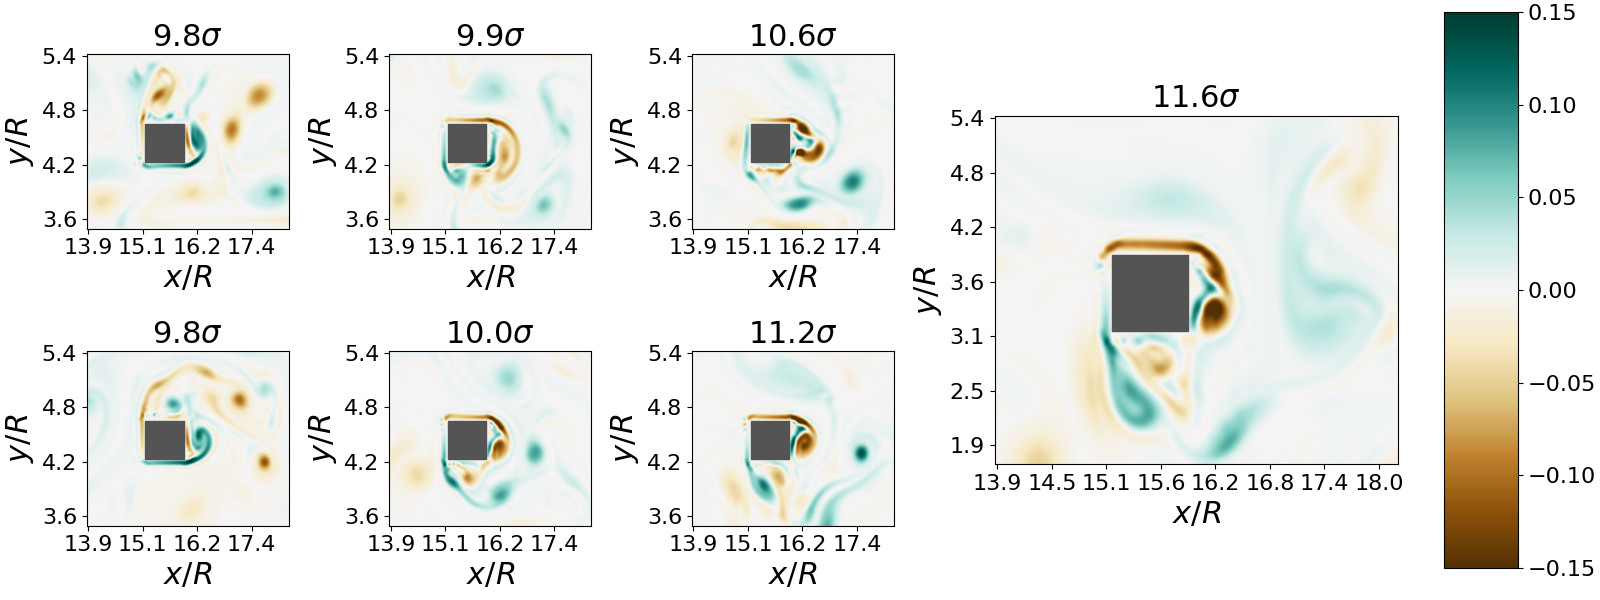
\includegraphics[width=\linewidth]{illustr_extrms_vorticity/illustr_extrms_vorticity.png}
  \caption{\label{fig:top_4_events_vorticity} Vorticity field (in lattice units) around the obstacle at $t=t^{\star}$ for the highest drag amplitudes recorded in the control run.
  }
\end{figure}

\begin{figure}
  \centering
  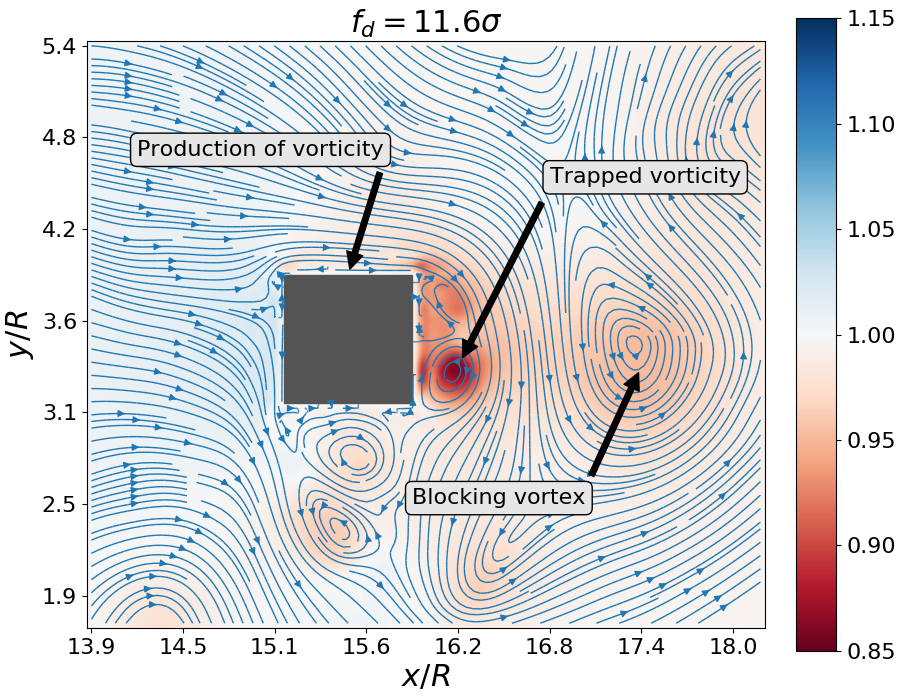
\includegraphics[width=.5\linewidth]{illustr_density_streamlines/illustr_density_streamlines.png}
  \caption{\label{fig:density+streamlines} Pressure field (in lattice units) and velocity streamlines at $t=t^{\star}$. In the near wake of the square, a (blocking) vortex blocks an intense vortex against the base of the obstacle. \EL{$f_d$ or $\tilde f_d$?}}
\end{figure}



\begin{figure}
  \centering
  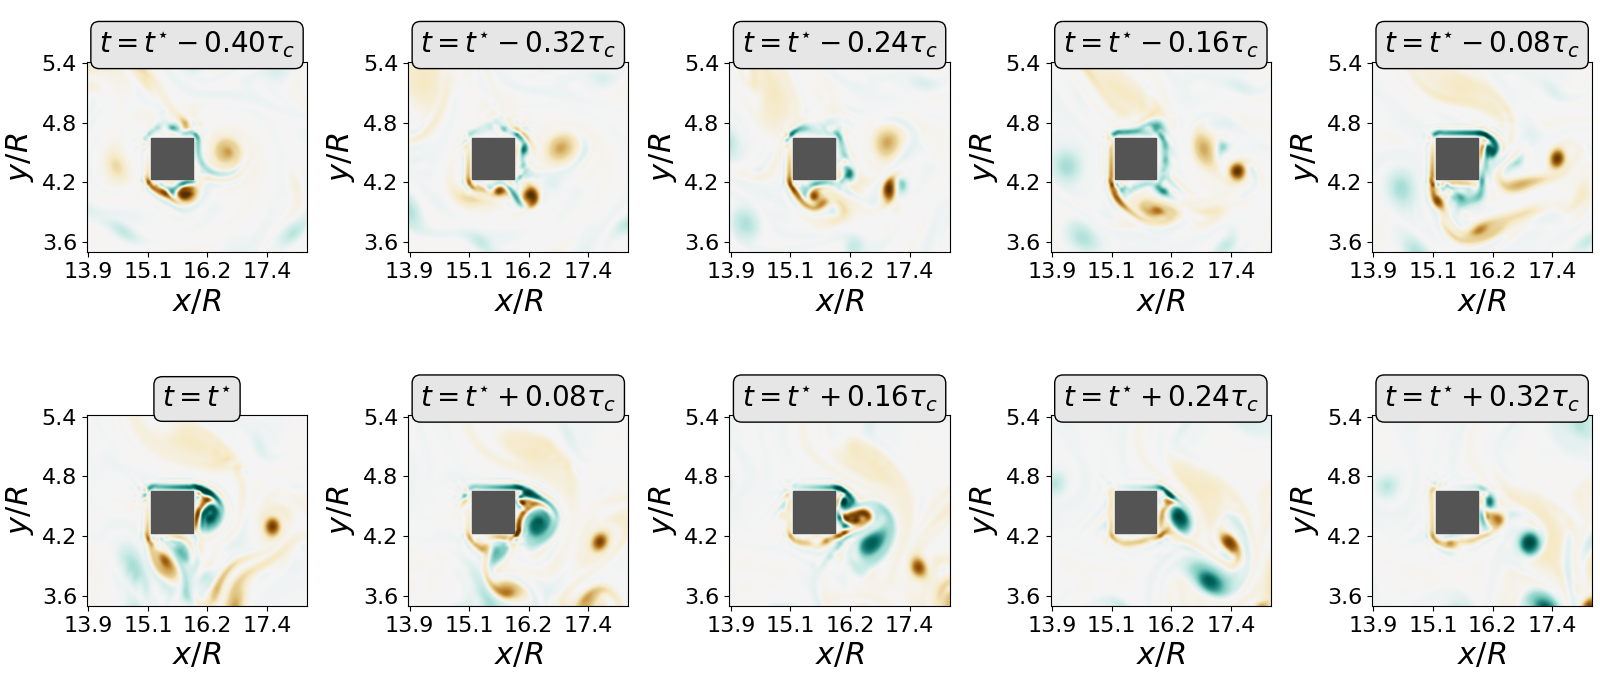
\includegraphics[width=.8\linewidth]{dynamics_extremes/dynamics_extremes.png}
  \caption{\label{fig:vorticity_dynamics} Snapshots of the vorticity field (in lattice units)  around $t=t^{\star}$.}
\end{figure}



% flow scenario
%
Fig.~\ref{fig:top_4_events_vorticity} displays the vorticity field (in lattice units) around the obstacle for the highest amplitudes of the drag during the control run.
%
In each case, an intense vortical structure is visible near the base of the obstacle.
The vorticity level of this structure is typically twice the amplitude of typical vorticity fluctuations observed in Fig.~\ref{fig:typical_vorticity}.
%
The formation of this vortex originates from an intense negative (positive) vorticity layer at the top (bottom) boundary of the obstacle. 
%
This high vorticity is responsible for a significant pressure drop at the base of the obstacle and, therefore, a strongly enhanced drag. In contrast, nothing special happens near the forebody of the obstacle.  


The high pressure drop on the base of the obstacle appears to be closely related to the presence of a strong vortex blocked against the base. 
As illustrated in Fig.~\ref{fig:density+streamlines}, this blockage is enforced by the presence of opposite vorticity in the near wake, which holds the vortex against the base of the obstacle and prevents him to be swept away downstream.
% 
This scenario is better evidenced in Fig.~\ref{fig:vorticity_dynamics}, where the time history of the vorticity field around $t=t^\star$ for the same event is shown. 
%
Before the occurrence of the extreme event, positive vorticity originating from the bottom boundary layer develops in the near wake of the square. This positive vorticity  prevents the shedding of negative vorticity and enforces the development of a intense vortex against the base of the square. 
When the blocking vortex is in turn advected downstream, the vortex against the base is released.
%
Consistently, one can argue that the typical duration of this scenario is related to the sweeping time of the flow past the obstacle, and is therefore of the order of $\tau_c$. 
This scenario is generic and has been observed for most extreme events sampled in the control run.

%We found that $80\%$ of the extreme events sampled from the control timeseries can be related to very similar dynamics.

\begin{figure}
	\centering
	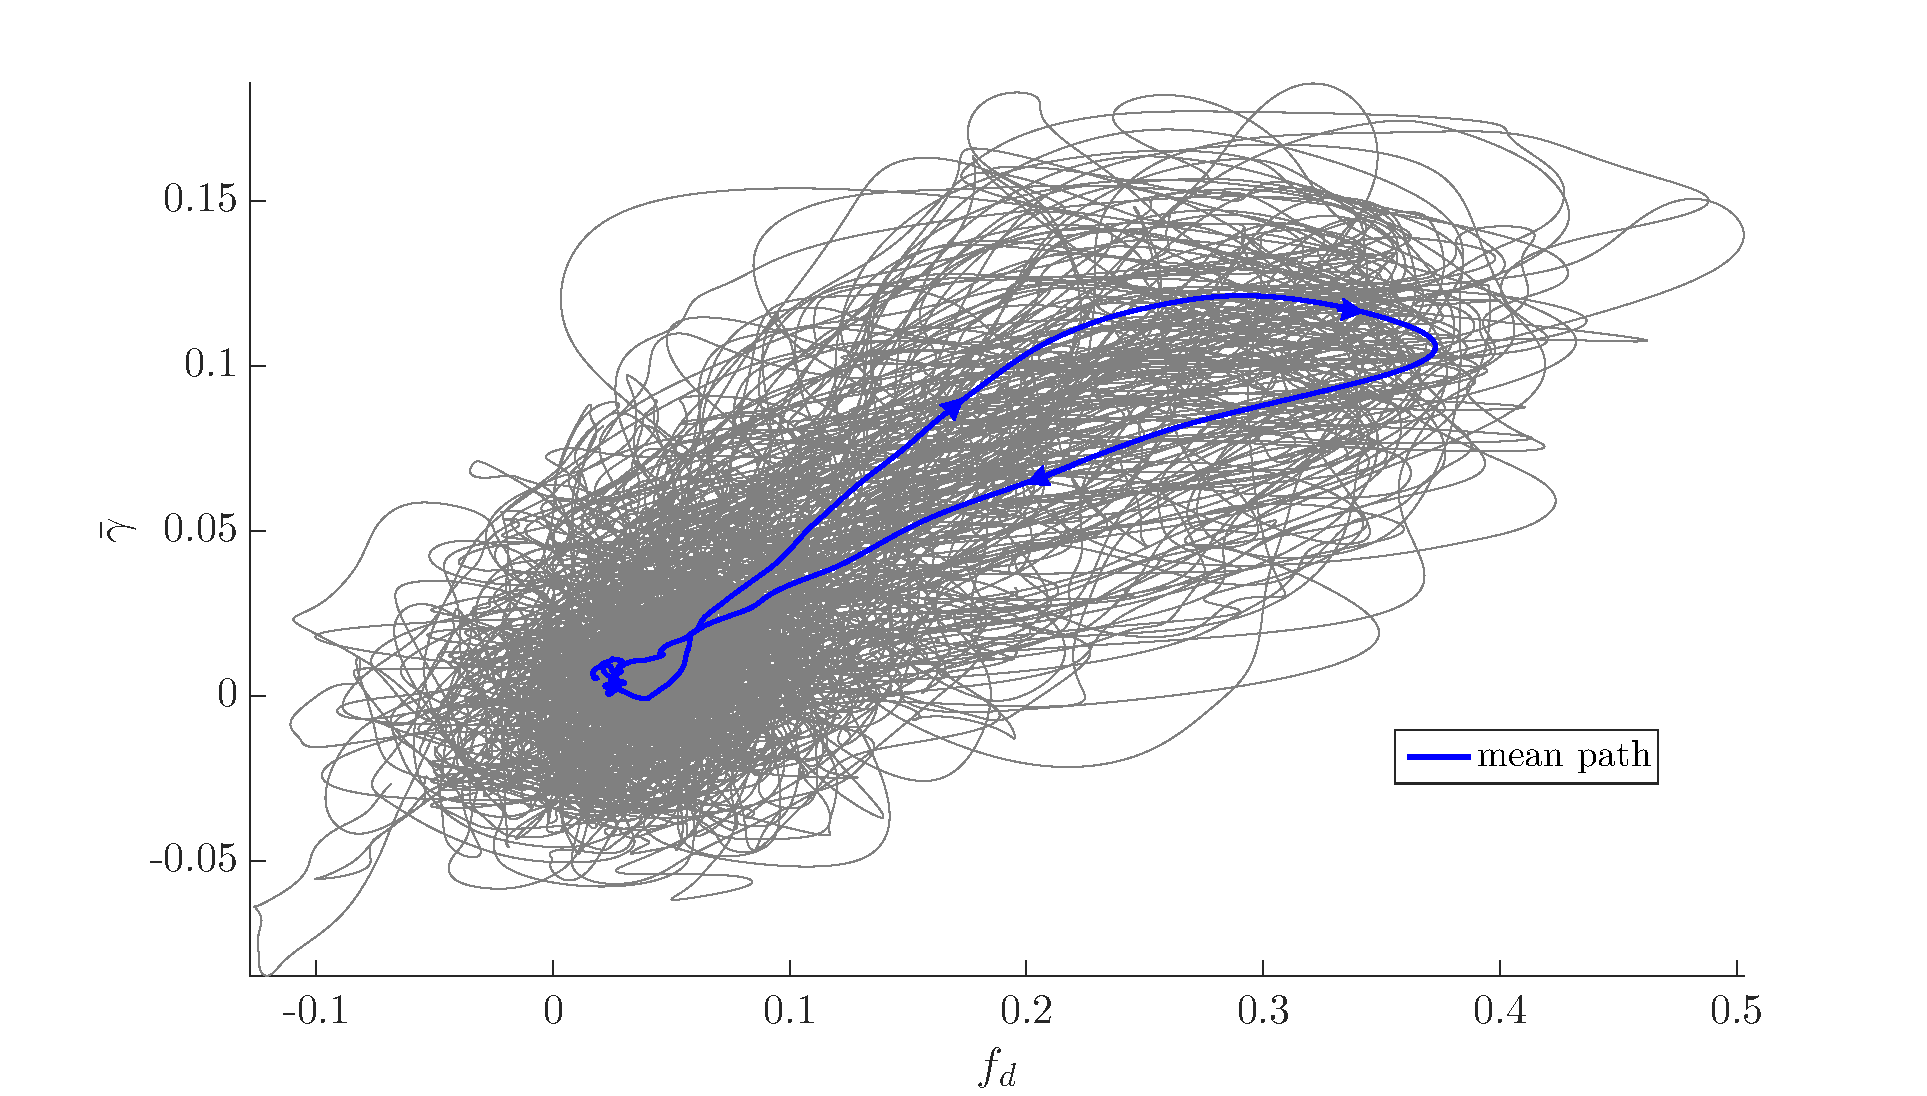
\includegraphics[width=.7\linewidth]{shear_asof_drag/shear_asof_drag}
	\caption{\label{fig:shear_asof_drag} Evolution of the (integrated) shear along the top or bottom sides of the obstacle as a function of the drag for $t^{\star}-2\tau_c \leq t \leq t^{\star}-2\tau_c$. Each trajectory corresponds to an event. The blue line is the mean path averaged over the set of extreme events sampled in the control run.}
\end{figure}


Since the occurrence of large drag amplitudes arises from the production of vorticity along the top or bottom side of the square, it is now proposed to characterize the dynamics of extreme events by their trajectory in the parameter space $(f_d(t), \bar{\gamma}(t))$ where $\bar{\gamma}(t)$ is the averaged shear along the top or bottom boundary of the square. Precisely, 
\begin{equation}
  \label{eq:avg_shear_def}
  \overline{\gamma} = \frac{1}{R} \int_{\mathcal{S}_\parallel} \frac{\partial u(\mathbf{x})}{\partial y}\mathrm{d}\mathbf{x}
\end{equation}
where $R$ denotes the size of the square, $u$ is the streamwise component of the velocity field and $\mathcal{S}_\parallel$ is the surface of either the top or the bottom boundary.
%
% Figure~\ref{fig:type_1_and_type_2_a} displays the label of the 104 sampled events, sorted according to the amplitude of the corresponding fluctuation.
% It illustrates that the dynamics corresponding to the large majority of events also corresponds to the events with the highest fluctuation amplitude.
%
Fig.~\ref{fig:shear_asof_drag} shows $\overline{\gamma}(t)$ as a function of the instantaneous drag $f_d$(t) for $t^{\star}-2\tau_c \leq t \leq  t^{\star}+2\tau_c$ for the sampled extreme events.
Before and after the extremal fluctuation, \textit{i.e.}  $t^{\star}-2\tau_c \leq t \leq t^{\star}-\tau_c$ and $t^{\star}+\tau_c \leq t \leq t^{\star}+2\tau_c$, paths wander in the region related to typical values of both $\overline{\gamma}$ and $f_d$.
On the contrary, the drag abruptly varies for $t^{\star}-\tau_c \leq t \leq t^{\star}+\tau_c$ near the extremal amplitude.
%Paths in the $(f_d, \bar{\gamma})$ space display excursions to atypical values for both $\bar{\gamma}$ and $f_d$.
These excursions always go clockwise, that is, $\overline{\gamma}$ attains its maximum value before $f_d$ does. 
This is consistent with an increase of $\overline{\gamma}$ acting as a precursor for extreme drag fluctuations in agreement with the previous description of flow scenarii.

%The remaining $20\%$ of the sampled events correspond to slightly different dynamics. In this case the vorticity responsible for the base pressure drop is not created along the top or bottom boundary, but directly through viscous shear alongside the base boundary of the obstacle. This viscous shear is induced by a large vortex detached from the obstacle. For a more detailed description of such dynamics, see chapter 3 of~\cite{lestang:tel-01974316}.



\subsection{Extreme fluctuations of the time-averaged drag }
\label{sec:time_avg}


\begin{figure}
	\centering
	%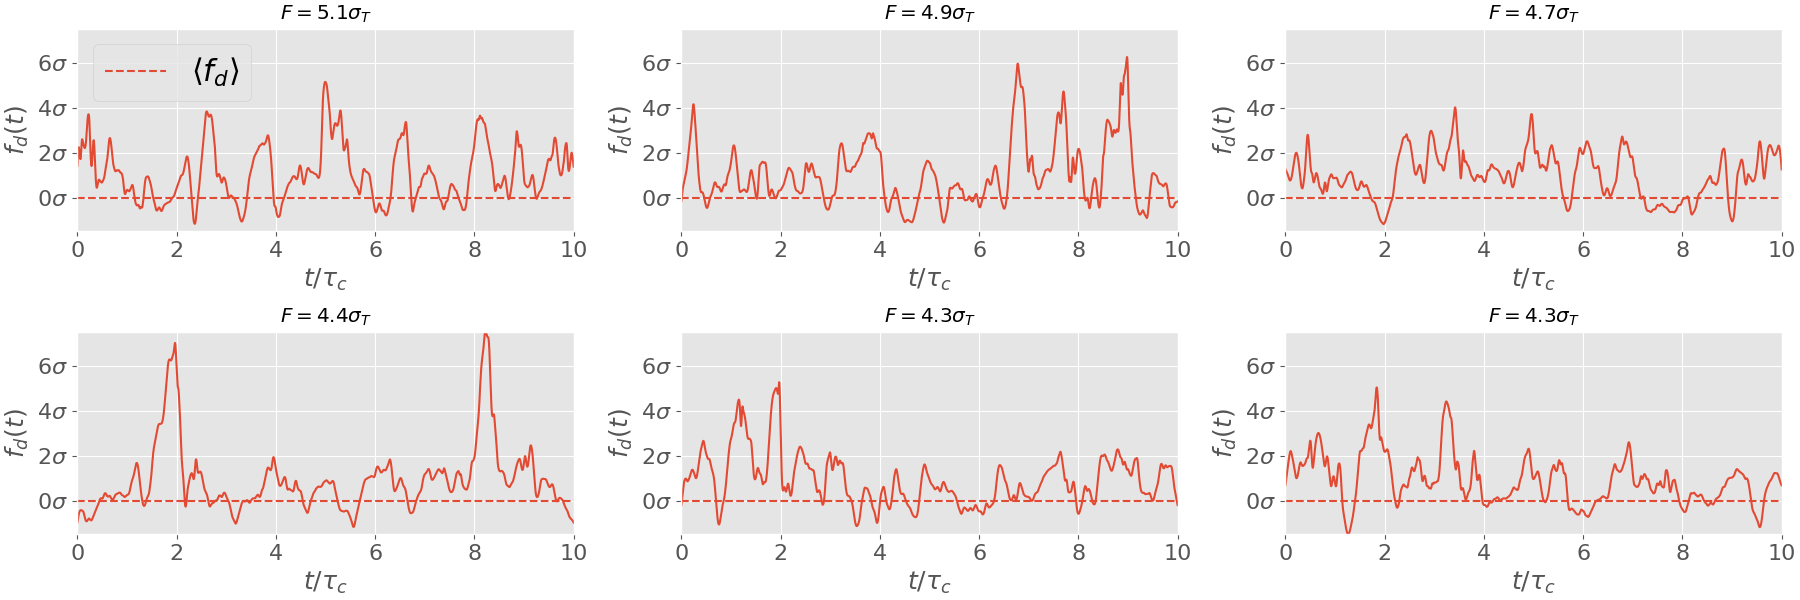
\includegraphics[width=\linewidth]{timeseries_extrms_AVG/timeseries_extrms_AVG}
	\caption{Instantaneous drag signals $f_d(t)$ corresponding to the highest fluctuations of the time-averaged drag $F_T$ with averaging period $T=10~\tau_c$ and $\tau_c$ being the correlation time of the drag. $\sigma_T$ denotes the standard deviation of $F_T$. \EL{FIGURE IS MISSING}}
	\label{fig:extreme_avg}
\end{figure}

% motivation
%
%In section~\ref{sec:instantaneous_drag}, we discussed the phenomenology of rare events corresponding to extremely high values of the drag acting on the square obstacle mounted in the flow described in section~\ref{sec:test_flow}. In particular, it was pointed out that such extreme drag fluctuations have a lifetime of, roughly, one correlation time $\tau_c$.
We discussed previously the phenomenology of extreme fluctuations of the \emph{instantaneous} drag and pointed out that the time scale associated with the development of such event was of the order of the sweeping time of the flow past the obstacle, or $\tau_c$. 
In practical applications, this duration may be much smaller than the characteristic response time of the material structure subject to these fluctuations.
% Consider for instance the interaction of a deformable structure with a turbulent flow: the typical response time may be much larger than the lifetime of drag fluctuations.
%
% definition
%
Therefore, a relevant observable is the \textit{time-averaged} drag
\begin{equation}
  \label{eq:def_time_averaged_drag}
  F_T(t) = \frac{1}{T}\int_t^{t+T} f_d(t) \mathrm{d}t,
\end{equation}
where $f_d(t)$ denotes the instantaneous drag and $T$ is the timescale (response time) of interest. We shall consider $T=10~\tau_c$ in the following.

During a time interval $[t;t+T]$, a fluctuation of $F_T(t)$ may be viewed as the overall contribution of roughly $T / \tau_c$ independent fluctuations of the {instantaneous} drag $f_d$.  
% phenomenology
%
% What is the phenomenology leading to extreme values of $F_T(t)$ ?
It is thus legitimate to ask whether a large value of the averaged drag results from (case (1)) a single outstanding fluctuation of the instantaneous drag,  or from (case (2)) a series of moderate positive fluctuations. 
%
%
The averaged drag signal $\{F_T(t)\}_{0 \leq t \leq T_{tot}-T}$ is obtained straightforwardly by filtering in time the instantaneous drag signal $f_d(t)$. 
In the same way as in section \ref{sec:extreme_extraction}, one can identify extreme fluctuations of $F_T$ exceeding some fixed threshold $a$ and sample a set of extreme events.
By taking $a=5.2~\sigma _T$  with $\sigma_T$ being the standard deviation of the fluctuations of $F_T$, $84$ independent extreme events have been selected.


% neither case (1) nor case (2)
%
Fig.~\ref{fig:extreme_avg} displays the timeseries $\{f_d(t)\}_{t^{\star} \leq t \leq t^{\star}+T}$ for several extreme fluctuations of $F_T$ occurring at $t=t^\star$.
It is established that extreme fluctuations of the time-averaged drag can neither be reduced to case (1) nor case (2). 
Indeed, both cases are featured in Fig.~\ref{fig:extreme_avg} along with mixed situations where very large value of the averaged-drag results from both a very large fluctuation and a significant succession of moderate (positive) fluctuations of the instantaneous drag.
%
% theoretical explanation
%
This observation may be explained by the exponential shape of the tail of the \ac{pdf} describing extreme positive drag fluctuations~\cite{lestang_computing_2018} (see Fig.~\ref{fig:pdf_drag}). 
Indeed, let $X$ be a random variable with \ac{pdf} $\mathbb{P}(X)$ and standard deviation $\sigma_X$.
Considering an extreme positive value of $S_N=\sum_{n=1}^{N}X_n$, the probability $p_1$ (resp. $p_2$) of case (1) (resp. case (2)) writes   
\begin{equation}
  \label{eq:indep}
  p_{1}  \left(\sum_{n=1}^{N} X_n = S_N\right) \propto \mathbb{P} \left(\frac{S_N}{N} \right)^{N} \quad \text{and} \quad p_{2}  \left(\sum_{n=1}^{N} X_n= S_N\right) \propto \mathbb{P}(S_N)  
\end{equation}
If $\mathbb{P}$ has an exponential positive tail, \textit{i.e.} $\mathbb{P}(X=x) \underset{x \gg \sigma_X}{\propto} e^{-\lambda x}$, both cases (1) and (2) have equivalent probabilities provided that the average $a=S_N/N$ is very large:
\begin{equation}
  \frac{p_{2}}{p_{1}} \underset{a\to \infty}{\to} \left(e^{\lambda a }\right)^{N} e^{-\lambda a N} = 1
  \label{eq:ratio_exp}
\end{equation}


\section{Rare-event algorithms}
\label{sec:rare_events_algorithms}

% limitation of direct sampling
%
In the limit of very rare events and complex dynamics (such as turbulent flows in industrial or environmental domains) the computational cost of  direct sampling becomes prohibitive. According to Eq.~\eqref{eq:return_time}, the return time of a fluctuation $f_d \geq a$ scales as $r(a) \propto e^{\lambda a}$.
As a consequence, the computational cost required to sample (directly) events of amplitude $f_d \geq a$ diverges exponentially as $e^{\lambda a}$.
%% objective
% In this section we discuss the application of \textit{rare event algorithms} to the numerical sampling of extreme drag forces on immersed objects, on the example of the flow presented in section~\ref{sec:test_flow}.
The motivation behind rare-events algorithms is to sample extreme fluctuations for a computational cost much lower than that related to return times.
%
For this purpose, the \acl{ams} (\ac{ams}) and \acl{gktl} (\ac{gktl}) algorithms are considered in the following.
%
%
Both algorithms consider an ensemble of $N$ trajectories $\{\mathbf{x}_n(t)\}_{0\leq t \leq T_a}$ with $n=1 \cdots N$, where each $\{\mathbf{x}_n(t)\}_{0\leq t \leq T_a}$ refers to a trajectory (of duration $T_a$) of the system in the phase space. In our case, the dynamical system under investigation is the flow described in section~\ref{sec:test_flow}.
In brief, the trajectories are replicated or discarded in the ensemble according to some \emph{selection rules} allowing us to sample more frequently rare events of some observables of interest, \textit{e.g.} the drag.
These selection rules are designed so that the introduced statistical bias is known at each iteration of the algorithm. The generated trajectories receive a weight whose knowledge makes it possible to calculate the probability and expectation values of the observables. 
% These two algorithms will be detailed in the following.

% In section~\ref{sec:ams}, we highlight that sampling  extreme fluctuations of the instantaneous drag with the \ac{ams} algorithm is a difficult task.
% In section~\ref{sec:gktl}, we apply an importance sampling algorithm, the \ac{gktl} algorithm, and efficiently sample rare trajectories corresponding to extreme fluctuations of the time-averaged drag.
% As an application, we use the \ac{gktl} algorithm to compute return times of very rare drag fluctuations.


\subsection{Extreme instantaneous drag forces with the \acl{ams} algorithm}
\label{sec:ams}

\begin{figure}
  \centering
  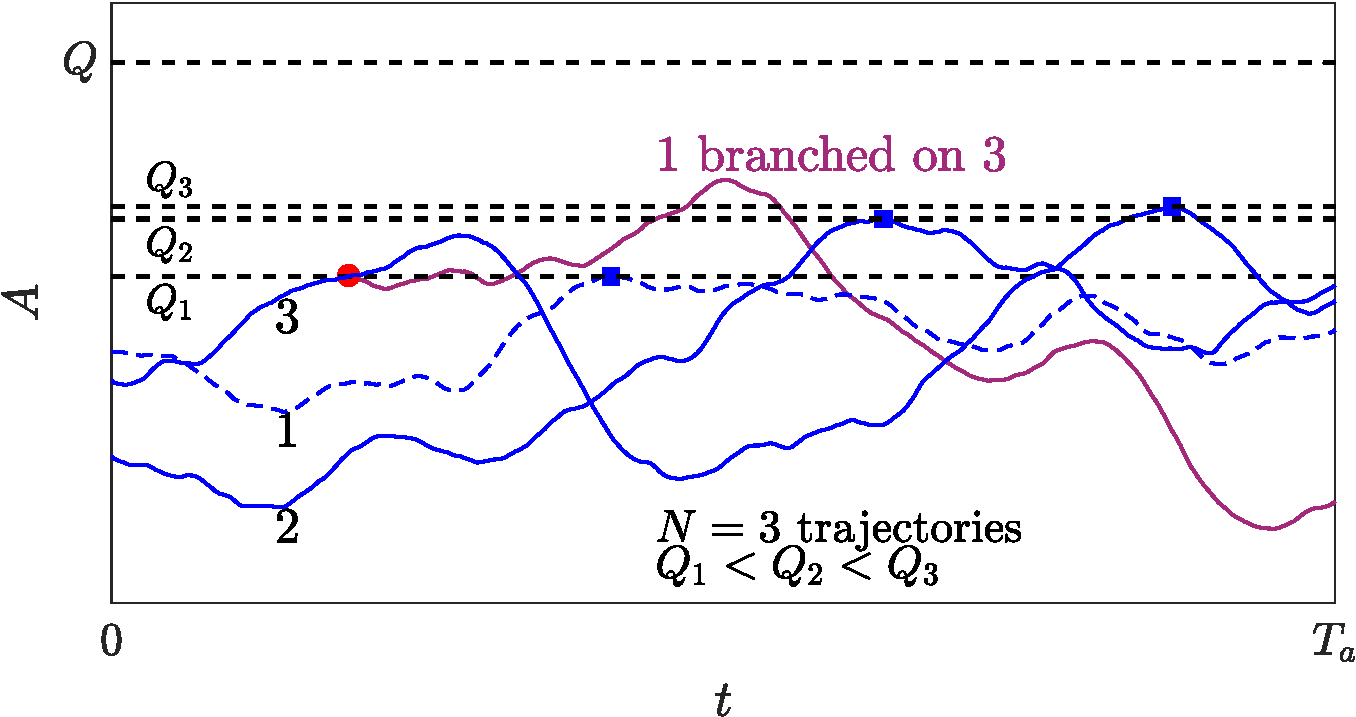
\includegraphics[width=.7\linewidth]{illustr_AMS/figure_AMS}
  \caption{\label{fig:illustr_AMS} Selection-mutation procedure of the \ac{ams} \EL{ou TAMS?} algorithm to compute the probability that a real-valued observable $A(\mathbf{x}(t))$ reaches values larger than $Q$ throughout a trajectory of duration $T_a$.\EL{QUID of the score function mentioned in the text: is the observable?} The initial ensemble of blue trajectories (associated with the time evolution of the observable $A$) is first generated. These trajectories are independent and can be simulated in parallel. On the basis of the respective maxima $Q_1$, $Q_2$ and $Q_3$, the trajectory with the lowest maximum is discarded in the ensemble (dashed blue line). Among the two remaining trajectories, trajectory 3 is chosen randomly and copied until it reaches the value $Q_1$. It is then freely simulated from the branching point to the final time $T_a$. In case of deterministic dynamics, a small perturbation is introduced at the branching to separate the trajectories. This procedure is iterated $J$ times or until all trajectories exceed a fixed threshold $Q$.}
\end{figure}

% Introduction of AMS
%
The \acl{ams} algorithm \cite{cerou_adaptive_2007} inherits the basic ideas of {splitting algorithms} \cite{KahnHarris1951}, in which the sampling of a rare event is made easier by splitting the dynamical path of the system (in phase space) into 
%a sequence of events that can be sampled with a higher probability  
a sequence of ``short-cuts'' that lead more rapidly to the realization of this event \cite{glasserman_multilevel_1999,rolland_statistical_2015}. The related selection-mutation step of this algorithm is sketched in Fig.~\ref{fig:illustr_AMS}.
%
% As already mentioned in the introduction, the \ac{ams} has been successfully applied to a large body of problems for the past ten years. 
%
% Over the past ten years the \ac{ams} has been successfully applied to a large body of problems, including the computation of the dissociation time of biomolecules~\cite{teo_adaptive_2016} or the simulation of rare relaminarizations in a stochastic model of wall turbulence~\cite{rolland_extremely_2018}.
%
% Quick description of TAMS
%
We consider here a variant \EL{generalization?} of \ac{ams} called \ac{tams}, in which the branching procedure relies on a time-dependent \textit{score function} $\xi (\mathbf{x}(t),t)$. Each iteration therefore consists in discarding the trajectories with the lowest maxima of the score function $\xi (\mathbf{x}(t),t)$ during the time interval $0\leq t \leq T_a$. Discarded trajectories are re-sampled according to the remaining trajectories.
% As an illustration, a particular iteration of the \ac{tams} algorithm is sketched in figure~\ref{fig:illustr_AMS} .
Further details about the algorithm and corresponding mathematical results are provided in \cite{lestang_computing_2018} and references therein.
\EL{What is the difference between AMS and TAMS? why do we need TAMS rather than AMS, This is not mentioned in text.} 

\subsubsection{Application of the \ac{ams} \EL{OR TAMS?} to a simple case: the \acl{ou} process}
\label{sec:ams_ou}

% Example: OU process
\begin{figure}
  \centering
  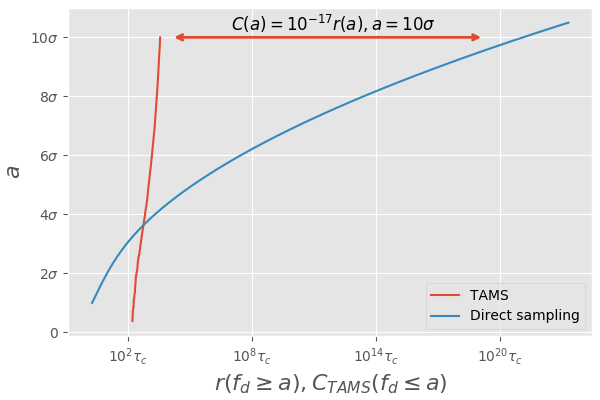
\includegraphics[width=.7\linewidth]{AMS_OU/AMS_OU.png}
    \caption{Efficiency of the \ac{tams} algorithm with respect to direct sampling in the case of an Ornstein-Uhlenbeck process \cite{lestang_computing_2018}. The orange line represents the evolution of the maximum obtained from re-sampled trajectories as a function of the computational cost $C_{TAMS}$. The solid blue line is the analytical solution for the return time of amplitude $a$. \EL{how many trajectories in the ensemble? REPLACE $f_d$ with $x$ in figure} }
  \label{fig:comparaison_temps_de_retour}
\end{figure}


Fluid dynamics is temporarily left aside and a one-dimensional \acl{ou} process is considered. This should allow us to highlight differences with fluid dynamics.
\begin{equation}
  \label{eq:ou}
  \dot{x} = -x + \sqrt{2\epsilon}\eta (t)  
\end{equation}


The \ac{tams} is applied  to a set of \EL{$N$} trajectories $\{x_n(t)\}_{0\leq t \leq T_a}$ with the objective to sample fluctuations of $x\geq a$ with $a$ being very large compared to typical values of $x$. The score function is here $x(t)$ and only one single trajectory is re-sampled at each iteration.
%
%Let $a_j$ be the maximum of the re-sampled trajectory at iteration $j$.
%
The computational cost of the algorithm after $J$ iterations is related to the simulation of the $N$ initial trajectories and the re-sampling of $J$ trajectories.
Fig.~\ref{fig:comparaison_temps_de_retour} compares the computational cost of the \ac{tams} algorithm with that of a direct sampling. 
In the latter, the typical computational cost is simply the return time $r(a)$.
Obviously, the successive re-samplings of the \ac{tams} algorithm lead very rapidly to trajectories exhibiting extreme fluctuations.
The related computational cost is many orders of magnitude lower than that of direct sampling.

Undoubtedly, the \acl{ou} process is an oversimplified dynamics to showcase the efficiency of the \ac{ams} or \ac{tams} algorithm.
Indeed, the state space is one-dimensional and the choice of the score function is straightforward. It is the process $x(t)$ itself.
In addition, the noise term in Eq.~\eqref{eq:ou} has no correlation in time, which implies that newly generated trajectories quickly separate from their parents.


\subsubsection{The \ac{ams} for extreme drag fluctuations}
\label{sec:ams_drag}

\begin{figure}
	\centering
	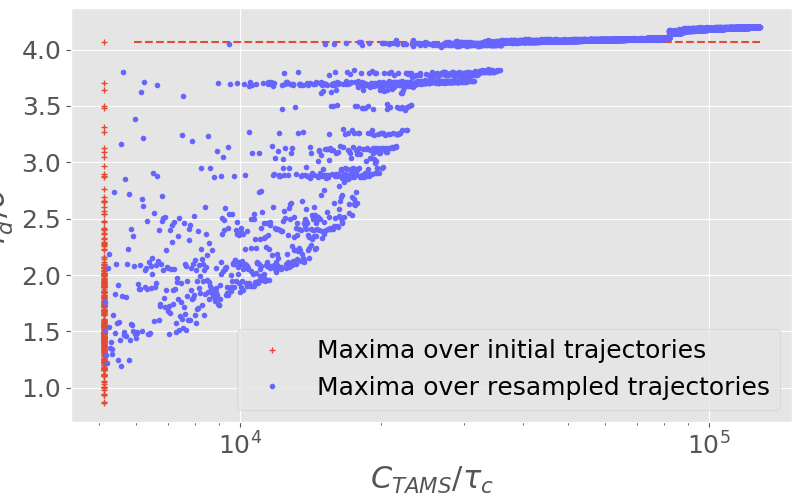
\includegraphics[width=.7\linewidth]{AMS_drag_resampling/AMS_drag_resampling.png}
	\caption{\label{fig:AMS_drag_resampling} Maximum of the instantaneous drag throughout the re-sampled trajectories as a function of the corresponding computational cost $C_{TAMS}$. The \ac{tams} is unable to efficiently sample rare trajectories associated to drag fluctuations higher than the largest fluctuation already captured in the initial ensemble.}
\end{figure}


% Application to instantaneous drag
%
% Can the \ac{tams} algorithm achieve similar performance when applied to complex chaotic dynamics, such as turbulent flows around objects ?
% To answer this question, we consider again the two-dimensional test flow introduced in section~\ref{sec:test_flow}.
%
Our aim is now to sample flow evolution that exhibit extreme fluctuations of the drag $f_d$ acting on the square obstacle.
In contrast with the \acl{ou} process, the phase space is here higlhy-dimensional with intrinsically chaotic dynamics.
In that situation, the choice of the score function $\xi (\mathbf{x}(t),t)$ is no longer straightforward.
However, a natural simple choice for which we will opt in this study is certainly $\xi (\mathbf{x}(t),t) = f_d(t)$. 
\EL{say something about the perturbation applied at branching?}


% application
%
The \ac{tams} is applied with $N=256$ trajectories of duration $T_a = 20\tau_c$.
%
Fig.~\ref{fig:AMS_drag_resampling} displays the maximum drag achieved by the re-sampled trajectories as a function of the computational cost, similarly to Fig.~\ref{fig:comparaison_temps_de_retour}.
%
%
The distribution of the maximal drag for the \textit{initial} trajectories is also shown.
After a few iterations, the trajectories with the lowest maxima of the score function are discarded, and new trajectories with higher maxima are re-sampled.
These maxima are depicted by the stars in Fig~\ref{fig:AMS_drag_resampling}.
Importantly, one can see that re-sampled trajectories never exceeds the amplitude of the highest maximum in the initial set of trajectories. This in contrast with the case of the \acl{ou} process. 


\begin{figure}
  \centering
  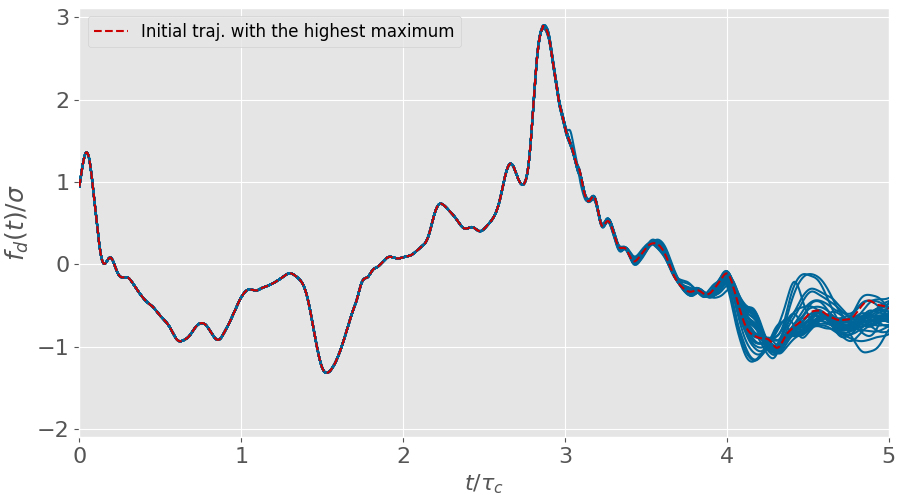
\includegraphics[width=.7\linewidth]{AMS_drag_trajectories/AMS_drag_trajectories.png}
  \caption{\label{fig:AMS_drag_trajectories} Ensemble of $N = 32$ trajectories after $181$ iterations of the selection-mutation procedure. In this experiment, the \ac{tams} algorithm is used with the instantaneous drag $f_d(t)$ as score function. Each trajectory has a duration $T_a = 5\tau_c$ (correlation time of the drag).
  The \ac{tams} fails to efficiently sample rare trajectories. All trajectories are eventually re-sampled from the trajectory displaying the highest maximum in the initial ensemble.}
\end{figure}

%pitfall
%
Fig.~\ref{fig:AMS_drag_trajectories} displays the ensemble of trajectories after many iterations of the \ac{tams} re-sampling procedure. 
%
Let us mention that for the sake of simplicity, the trajectory of the system is  here abusively associated with the time evolution of the observed drag.  \EL{useful to mention?}
%
Interestingly, it is obtained that all trajectories ultimately originate from one unique initial trajectory. 
%
This feature may be explained as follows.
Because the dynamics has a memory, it takes a certain time before a re-sampled trajectory separates from its parent. In our situation, this memory originates from the deterministic nature of fluid dynamics. 
Two trajectories (of the drag signal) starting from infinitesimally close points typically overlap over a timescale $\tau_L$ called the \textit{Lyapunov timescale}~\cite{lyapunovRef}. \EL{Freddy: Provide citation for Lyapunov timescale}
%
In our case, we observe in Fig.~\ref{fig:AMS_drag_trajectories} that the duration of extreme drag fluctuations is shorter than the Lyapunov timescale of the drag process.
Therefore, the re-sampling of a trajectory branched at $t=t^{\star}$ corresponding to the maximal drag amplitude cannot lead to larger values for $t^{\star} \leq t \leq t^{\star}+\tau_L$. For $t - t^{\star} >\tau_L$, the drag process has lost the memory of the drag fluctuations on which the re-sampling was based. Therefore, the probability of observing a new extreme fluctuation is also very low.
%

The difference between the typical duration of drag fluctuations $\tau_c$ and the Lyapunov timescale $\tau_L$ may be heuristically associated with the ``convective nature'' of the flow.
%
As discussed previously, the duration of extreme fluctuations of the drag are closely related to the sweeping time of the flow past the obstacle, and therefore to the mean velocity $U$. On the contrary, the Lyapunov timescale is rather associated with the intrinsic evolution of turbulent fluctuations in the reference frame of the mean flow, \textit{i.e.} with the fluctuating velocity $u_{rms}$. The ratio $u_{rms}/U < 1$ in our case of grid-generated turbulence implies that $\tau_L > \tau_c$. \EL{does it make sense to you?}
 
%As discussed previously, extreme fluctuations of the drag $f_d$ have a lifetime of length roughly $\tau_c$.  Fluid structures responsible for a particular value of the drag on the obstacle at a time $t^{\star}$ are swept away by the mean flow over a timescale $\tau_c$, shorter than the time it takes for trajectories to separate, \textit{i.e} the Lyapunov timescale. 


% perspectives
%
In summary, it appears that a straightforward application of the \ac{tams} by taking the drag as score function does not allow us to efficiently sample extreme fluctuations.
%
Indeed, there is \textit{a priori} no reason for the drag itself to be a good indicator of how likely next drag fluctuations will develop.
On the other hand, finding a better score function would require an intricate understanding of the flow scenario leading to extreme events, certainly beyond the phenomenological description developed in section~\ref{sec:dynamical_aspects}.
%
%Furthermore, such ``tuning'' is problem dependent.
%
A line of improvement might be to explicitly account for ``the correlation time of the observable being smaller than the Lyapunov time of the system'' by re-sampling the trajectories at a Lyapunov time \textit{before} the maximum is reached. That way, new events associated to higher fluctuations may have the opportunity to develop.
However, such modification of the procedure must be implemented with care, so as to preserve the mathematical properties (evaluation of the statistical bias) of the algorithm.
% 

\subsection{Extreme time-averaged drag forces with the \acl{gktl} algorithm}
\label{sec:gktl}

The sampling of extreme fluctuations of the time-averaged drag $F_T$ is now examined.
The \ac{tams} algorithm could be used in the same way as before by choosing $F_T$ as score function. However, this would lead to the same pitfall.
% the re-sampling fails to efficiently generate new higher fluctuations of $F_T$.
%
For a time-averaged observable,  an alternative approach is provided by the \acf{gktl} algorithm \cite{giardina_direct_2006,tailleur_probing_2007,giardina_simulating_2011}.
%
Similarly to the \ac{tams} algorithm, the \ac{gktl} algorithm relies on the simulation of an ensemble of trajectories.
In this case, however, the trajectories interact dynamically. 
%
At regular time intervals, some elements of the ensemble are killed and others are cloned according to a weight that depends on the history of the replica.
%
The weights are chosen so that, after several iterations of the algorithm, the trajectories generated are distributed according to a biased probability distribution in favor of trajectories with large values of the (time-averaged) observable of interest.
%
The \ac{gktl} algorithm belongs to a family of algorithms called ``go with the winners'' \cite{aldous1994go,grassberger2002go}.
Similar ideas have been applied in a wide range of fields over the past 50 years, under different names \EL{donner des exemples}, depending of the specific application domain~\cite{moral_feynman-kac_2004}.
The application of a go-with-the-winners approach to the computation of large deviations in non-equilibrium systems has first been proposed in 2006 \cite{giardina_direct_2006}.
Over the past ten years, it has successfully been applied to investigate rare events in both stochastic \cite{giardina_direct_2006,lecomte_numerical_2007,garrahan2007dynamical} and deterministic systems \cite{giardina_direct_2006,tailleur_probing_2007}.
% It was originally designed to compute large deviations rate functions of time-averaged dynamical observables, that describe the probability density of both typical of rare events in the limit of large
% averaging time~\cite{ref_large_dev}.
% By contrast with the \ac{ams} and \ac{tams}, the \ac{gktl} algorithm does not follow the strategy of splitting algorithms.
% Instead, it implements \textit{importance sampling}, \textit{i.e.} sampling a modified distribution that is biased towards the rare events of interest.
% The idea of importance sampling is very general and was used in many different contexts (see e.g.~\cite{Berg1992,Hartmann2002} and the general references~\cite{Bucklew2004,RubinoTuffin2009}). 
% The \ac{gktl} algorithm performs importance sampling in the space of trajectories, which is relevant for out-of-equilibrium systems.

\subsubsection{The \ac{gktl} algorithm}
\label{sec:gktl_description}
As with the \ac{tams} algorithm, the \ac{gktl} algorithm is based on the simulation of an ensemble of $N$ trajectories $\left\{\mathbf{x}_{n}(t)\right\}_{0\leq t \leq T_a}$ with $ n =1 \cdots N$ starting from independent random initial conditions.
%
Let us consider a real-valued observable of interest $A(\mathbf{x}(t))$ and introduce a cloning period $\tau$.
%
At time instants $t_{i}=i\tau$ with $i=1,~2,~...,~T_{a}/\tau$ ($T_{a}$ is a multiple of $\tau$) a weight $W_{n}^{i}$ is assigned to each trajectory. This weight is defined ($t_0=0$) by
%
\begin{equation}
W_{n}^{i}=\frac{e^{k\intop_{t_{i-1}}^{t_{i}}A(\mathbf{x}_{n}(t))dt}}{R_{i}}\quad \mbox{with the normalization factor} \quad R_{i}=\frac{1}{N}\sum_{n=1}^{N}e^{k\int_{t_{i-1}}^{t_{i}}A(\mathbf{x}_{n}(t))dt}
\label{eq:Weight}
\end{equation}
so that $\sum_{n=1}^N W_n^i = N$.
%
%
Therefore, the weights $\{W_{n}^{i}\}_{n=1\cdots N}$ determine (on average \EL{vague?}) how many copies of each trajectory are produced at time $t=t_i$. 
% For each t $\{\mathbf{x}_{n}\}_{0 \leq t \leq  t_i}$, a random number of copies of the trajectory are generated. This number is on average proportional to the weight $W_{n}^{i}$, such that the total number of trajectories produced at each event is equal to $N$.
%
For deterministic systems, a small perturbation is applied to the clones so that they can rapidly separate from their parents. 
%
% The parameter  is chosen by the user in order to control the strength of the selection.
%
The free parameter $k$ drives the amplitude of fluctuations targeted by the biased ensemble of trajectories.
A higher value of $k$ gives a higher weight to higher fluctuations and thus drives the sampling to more extreme events.


Let 
$\mathbb{P}_{0}\left(\left\{ \mathbf{X}(t)\right\} _{0\leq t\leq T_{a}} = \left\{ \mathbf{x}(t)\right\} _{0\leq t\leq T_{a}}\right)$ 
refer formally to the probability of the trajectory 
$\left\{ \mathbf{x}(t)\right\} _{0\leq t\leq T_{a}}$ of our dynamical system.
%
% $\mathbb{P}_{k}\left(\left\{ \mathbf{X}(t)\right\} _{0\leq t\leq T_{a}} = \left\{ \mathbf{x}(t)\right\} _{0\leq t\leq T_{a}} \right)$ 
%
By construction, the probability to obtain the same trajectory by resorting to the previous cloning procedure is given by
%
\begin{align}
\mathbb{P}_{k}\left(\left\{ \mathbf{X}(t)\right\} _{0\leq t\leq T_{a}}=\left\{ \mathbf{x}(t)\right\} _{0\leq t\leq T_{a}}\right) &\underset{N\rightarrow\infty}{\sim} \frac{e^{k\int_{0}^{T_{a}}A(\mathbf{x}(t))dt}}{Z(k,T_a)}\mathbb{\mathbb{P}}_{0}\left(\left\{ \mathbf{X}(t)\right\} _{0\leq t\leq T_{a}}=\left\{ \mathbf{x}(t)\right\} _{0\leq t\leq T_{a}}\right)
\label{eq:Biased_Path_Approximation}
\end{align}
where the normalization factor is given by $Z(k,T_a)=\mathbb{E}_{0}\left[e^{k\int_{0}^{T_{a}}A(\mathbf{X}(t))dt}\right]$ with $\mathbb{E}_{0}$ being the expectation value with respect to $\mathbb{P}_{0}$.
%
% obvious? 
%and $\underset{N\rightarrow\infty}{\sim}$ meaning that this is true only asymptotically for large $N$.
%
%
%The typical error is of order $1/\sqrt{N}$ when evaluating averages over observables.
%
Eq.~\eqref{eq:Biased_Path_Approximation} relies on the mean-field approximation
\begin{equation}
R_{1}=\frac{1}{N}\sum_{n=1}^{N}e^{k\int_{t_0}^{t_{1}}A(\mathbf{X}_{n}(t))dt}\underset{N\rightarrow\infty}{\sim} Z(k,t_1)= \mathbb{E}_{0}\left[e^{k\int_{t_0}^{t_{1}}A(\mathbf{X}(t))dt}\right]
\label{eq:Mean_Field_Approximation}
\end{equation}
which by induction (and assuming similar relations for the successive $R_i$'s) eventually leads  to~\cite{giardina_direct_2006,giardina_simulating_2011}
\begin{equation}
\prod_{i=1}^{T_{a}/\tau}R_{i}\underset{N\rightarrow\infty}{\sim} Z(k,T_a) =\mathbb{E}_{0}\left[e^{k\int_{0}^{T_a}A(\mathbf{X}(t))dt}\right].\label{eq:Estimate_Lambda}
\end{equation}
\EL{IS IT TRUE?}
The validity of this mean-field approximation and the typical relative error related to this approximation being of order $1/\sqrt{N}$ have been proven rigorously \cite{DelMoralBook,DelMoral2013} for a family of rare-event algorithms including the \ac{gktl} algorithm.
%
%
The killed trajectories, \emph{i.e.} with a weight smaller than $1$ \EL{true?}, are discarded from the statistics.
%
% no because the trajectories are cloned
%
% Starting from the final $N$ trajectories at time $T_{a}$, one goes backwards in time through the selection events attaching to each piece of trajectory its ancestor.
%
Eventually, an effective ensemble of $N$ trajectories for $0 \leq t \leq T_{a}$ is obtained, distributed according to $\mathbb{P}_{k}$.
All trajectories are solutions of the dynamical system since we have not modified the dynamics, but only sampled trajectories according to the distribution $\mathbb{P}_{k}$ rather than according to the distribution $\mathbb{P}_{0}$.
\EL{quid the small perturbation to separated the clones? comment required}
%
The sampled trajectories can be used to compute the statistical properties of any observable with respect to the distribution $\mathbb{P}_{0}$ from the distribution $\mathbb{P}_{k}$ by using Eq.~\eqref{eq:Biased_Path_Approximation}.
%
More details concerning the implementation of the algorithm and the corresponding data analysis are provided in \cite{lestang:tel-01974316,brewer2018efficient}.

%
%\EL{next paragraph needs rephrasing or suppress}
%
%For instance, the expectation value of the observable $O\left(\left\{ \mathbf{X}(t)\right\} _{0\leq t\leq T_{a}}\right)$ is given by
%\begin{equation}
%\mathbb{E}_{0}\left[O\left(\left\{ \mathbf{X}(t)\right\} _{0\leq t\leq T_{a}}\right)\right]\underset{N\rightarrow\infty}{\sim}\frac{1}{N}\sum_{n=1}^{N}O\left(\left\{ \mathbf{X}_{n}(t)\right\} _{0\leq t\leq T_{a}}\right){e}^{-k\int_{0}^{T_{a}}A(\mathbf{X}_{n}(t))dt}{e}^{T_{a}\lambda(k,T_{a})},\label{eq:GK_O_estimator}
%\end{equation}
%where the $X_{n}$ are the $N$ backward reconstructed trajectories.
%Events that can be considered rare with respect to $\mathbb{\mathbb{P}}_{0}$ are oversampled following $\mathbb{P}_{k}$. As a result, the effective ensemble of trajectories generated by the \ac{gktl} algorithm contains a larger amount of such events, and empirical estimators such as~\eqref{eq:GK_O_estimator} have a dramatically lower statistical error.


\subsubsection{Application of the \ac{gktl} algorithm to extreme fluctuations of the time-averaged drag}
\label{sec:gktl_drag}

\begin{figure}
	\centering
	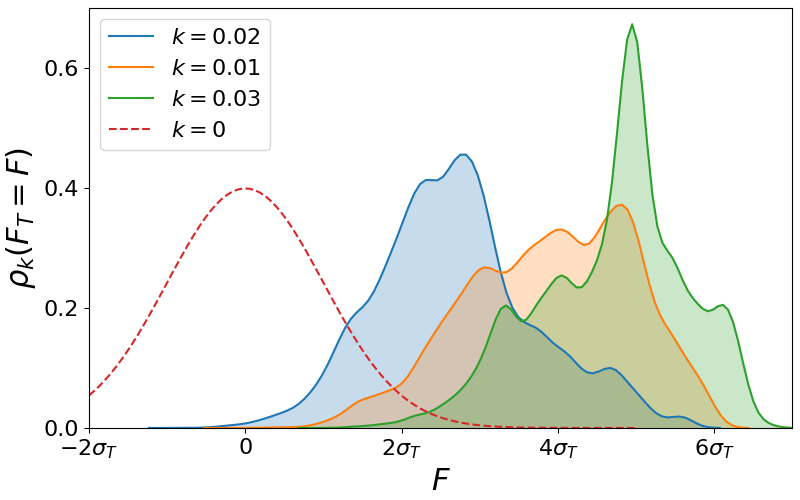
\includegraphics[width=0.7\linewidth]{IS_GKTL/IS_GKTL}
	\caption{\label{fig:IS_GKTL} Rare-event sampling of the (zero-mean) time-averaged drag $\tilde F_T = F_T - \overline{F_T}$ with $T=10~\tau_c$; $\tau_c$ is the correlation time of the instantaneous drag. The shaded \ac{pdf}s are estimated from the biased ensemble resulting from the \ac{gktl} algorithm applied to $16384$ trajectories of duration $T_a=T$ with the cloning period $\tau=\tau_c/2$.
	The dashed line denotes the unbiased \ac{pdf} of $\tilde F_T$, \textit{i.e.} from direct sampling or with $k=0$ (no bias) in the \ac{gktl} algorithm.
\EL{$F_T-\overline{F_T}$ in the figure!}}
\end{figure}

The application of the \ac{gktl} algorithm is now studied for the flow dynamics introduced in section~\ref{sec:test_flow} with the aim of sampling trajectories with extreme fluctuations of the \textit{time-averaged} drag.

% Choice of parameters and perturbation
The computational cost $C_{gktlS}$ depends on both the duration of each trajectory and the number of trajectories: $C_{gktl} = N \times T_a$.
In practice, $N=16384$ and $T_a = T = 10\tau_c$ which yields $C_{gktl} \approx 1.6 \times 10^5 \tau_c$.
A cloning period $\tau$ that is too short can result in a loss of information if the clones do not separate from their parents between two cloning steps. On the contrary, choosing $\tau \gg \tau_c$ may result in insufficient cloning steps to allow for efficient importance sampling.
As a result, a rule of thumb is to set $\tau \approx \tau_c$. We took $\tau = \tau_c /2$.
%
Three numerical experiments corresponding to three different values of the parameter $k$ have been performed.
%
%
%Let us remark that the value of $k$ should be chosen empirically unless a \textit{large deviation regime} $T_a \to \infty$ is verified  \cite{touchette_large_2009}.
%In the latter case, the parameter $k$ can be related to the typical amplitude of the sampled fluctuations through the Gartner-Ellis theorem \cite{touchette_large_2009}.
%
%
As a proof of realizability, Fig.~\ref{fig:IS_GKTL} displays the estimate of the biased \ac{pdf}s of the (zero-mean) time-averaged drag, $\tilde F_T \equiv F_T - \overline{F_T}$:
\begin{equation}
  \label{eq:estimate_biased_measure}
  \rho_k(F) 
  %= \mathbb{E}_{\mathbb{P}_k}[\delta(\tilde F_T(\{\mathbf{x}\}_{0\leq t \leq T_a})-F)]
  \approx \frac{1}{N}\sum_{j=1}^{N}\delta(\tilde F_{T}(\{\mathbf{x}_j\}_{0\leq t \leq T_a}) - F)
\end{equation}
in addition to the unbiased \ac{pdf} based on the control run.
%Note that the unbiased \ac{pdf} could also be estimated using the \ac{gktl} algorithm with $k=0$.


% limitations
%
For a fixed number of trajectories $N$, there is necessarily an upper limit $k_{max}$ over which the finite number of trajectories becomes detrimental to the efficiency and accuracy of the selection procedure.
%
indeed for $k \gtrsim k_{max}$, the re-sampling relies on a small number of ``independent trajectories'' and most of the trajectories (in the biased ensemble) overlap. 
This effect is highlighted in Fig.~\ref{fig:IS_GKTL} where the biased \ac{pdf} corresponding to $k=0.03$ is over-peaked.
%
Such finite-size effect is expected to gradually increase as the bias amplitude  $k$ is increased.
%
An important question concerning the application of the \ac{gktl} algorithm is therefore that of the dependence of $k_{max}$ on the ensemble size $N$. 
This point has been very recently examined in \cite{nemoto2017finite,Guevara_Hidalgo_2018}.
% how to assess the value of k_max ?
In this study, the order of magnitude of $k_{max}$ has been estimated \emph{empirically} by evaluating the diversity of the trajectories in the biased ensemble.
This diversity may be monitored at each selection step of the algorithm by calculating the proportion of trajectories sharing the same ancestor trajectory.

\begin{table}
	\centering
	\begin{tabular}{|l|c|c|c|c|c|}
		\hline
		& $\sigma$ & $2\sigma$ & $3\sigma$ & $4\sigma$ & $5\sigma$ \\
		\hline
		$k=0.02$ & ~1594~ & ~799~ & ~155~ & 22 & 0  \\ 
		\hline
		$~k=0.025~$ & 1019 & 834 & 521 & 198 & 27  \\ 
		\hline
		$k=0.03$ & 539 & 510 & 391 & 205 & 36  \\ 
		\hline
		${N}_{direct}$ & 2599 & 37 & 22 & ~0.5~ & ~0.005~ \\
		\hline
	\end{tabular}
	\caption{Number of fluctuations $F_{T} \geq a$ with a=$\sigma,~2\sigma,~...$ captured in the biased ensemble for $k=0.02,~0.025$ and $0.03$.
		Note that trajectories that overlap for more than half of their duration are counted as one.
		${N}_{direct}$ is the number of fluctuations expected from the direct sampling of $N$ independent realizations of $F_{T}$ of the same duration.}
	\label{tbl:nbTraj_tbl}
\end{table}

% Comparisons with direct sampling
%
The efficiency of the \ac{gktl} algorithm is now assessed with respect to direct sampling. 
Table~\ref{tbl:nbTraj_tbl} indicates the number of trajectories that correspond to a time-averaged $F_{T} \geq a$ for the different values of the bias parameter $k$.
Note that trajectories that overlap for more than half of their duration are counted as one.
%\footnote{Trajectories that overlap over an interval $[O;t]$ with $t\geq T_a / 2$.}
Table~\ref{tbl:nbTraj_tbl} also indicates the expected number of fluctuations one can expect from simulating $N$ independent trajectories $\{F_T(t)\}_{0\leq t \leq T_a}$, \emph{i.e.} with the same computational cost $C_{gktl}$.
%
%This number assumes that the values of the time-average drag $F_T$, with $T=10\tau_c$, are Gaussian distributed. This hypothesis is motivated by Fig.~\ref{fig:PDF_AVG}.



%\begin{figure}
%  \centering
%  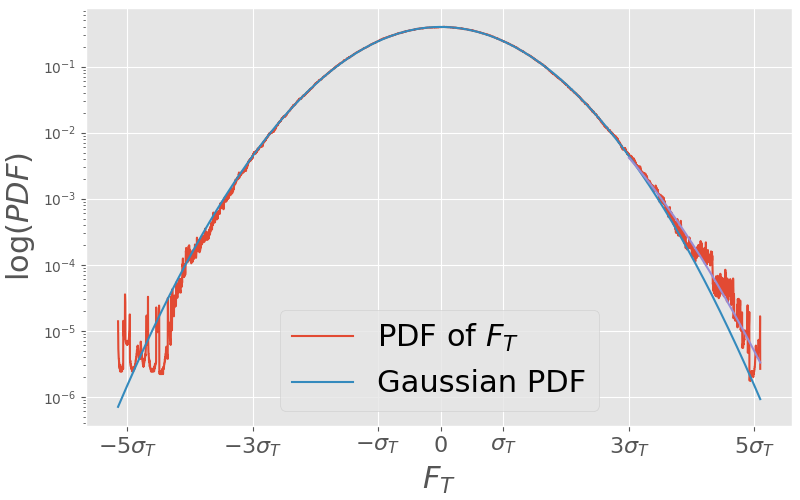
\includegraphics[width=.7\linewidth]{PDF_AVG/PDF_AVG}
%  \caption{PDF of average drag over $10\tau_c$}
%  \label{fig:PDF_AVG}
%\end{figure}

% Conclusion
%
Table~\ref{tbl:nbTraj_tbl} shows that the \ac{gktl} algorithm is able to sample drag fluctuations that are far from reach from a direct sampling approach of similar computational cost.
In section~\ref{sec:time_avg} we observed that extremely large values of the time-averaged drag can either result from a succession of rather typical---however all positive---fluctuations of the instantaneous drag $f_d$, or from a small number of extremely large fluctuations of the instantaneous drag.
By selecting trajectories based on the previous average value of the drag over a duration $\tau \approx \tau_c$, the \ac{gktl} algorithm is well suited for the preferential selection of trajectories of the former kind.
However, such selection strategy does not appear equally as favourable to trajectories of the latter type, for which all of the drag density is located in one or two vert large fluctuations of the instantaneous drag.
Further works must now investigate the nature of the sampled trajectories, and determine the amount of discrepancy concerning their respective phenomenology.


\EL{rajouter le calcul des temps de retour par gktl pour etoffer un peu la partie du papier sur gktl -- il faudrait montrer un resultat qui montre que l'on obtient la bonne statistique}

\section{Conclusion}
\label{conlusion}

\EL{CONCLUSION TO BE REVIEWED}

We assessed the application of two rare event algorithms for the numerical simulation of extreme mechanical efforts on structures immersed in a turbulent flow, a situation relevant to many industrial applications.
\\
In a first part, we investigated the dynamics and statistics of extreme fluctuations of the drag acting on a square mounted in a turbulent channel flow, in two dimensions.
By means of very long simulations---without rare event algorithm---we observed that such extreme events are caused by the concentration of vorticity very close to the base of the square.
Because of the sweeping of the fluid structure responsible for such a situation, extreme drag levels do not persist over time.
The lifetime of extreme drag fluctuations is of the order of the turnover time, and the corresponding drag signal is very peaked around the extreme value.
Our long drag timeseries also reveal that the tails of the \ac{pdf} for the drag are very well described by an exponential \ac{pdf}.
This property can be linked to the phenomenology of extremes of the time-averaged drag.
Indeed, we observed that such extreme values for the average do not preferentially result from a small number of very large fluctuations or an exceptional succession of typical fluctuations that
add up forming an extremely large value of the average.
Such a phenomenology can be described by a stochastic process with an exponential \ac{pdf}.
\\
On the basis of the same two-dimensional test flow, we then applied the \ac{ams} algorithm choosing the drag itself as a score function.
In this case, our results illustrate that the selection-mutation procedure is unable to generate rare trajectories at a better rate than a direct sampling approach.
This can be related to the phenomenology of extreme drag fluctuations, which lifetime is shorter than the timescale over which resampled trajectories separate from their parent following the
addition of a small perturbation in the initial conditions.
The \ac{gktl} has been applied to the sampling of trajectories displaying extreme fluctuations of the time averaged drag.
In this case, we showed that using the \ac{gktl} leads to a tremendous improvement with respect to a direct approach, allowing the simulation of trajectories that are out of reach without algorithm.
\\
The application of rare event algorithms relies on the definition of a score function, on which the selection of trajectories is based upon.
Although the dynamics itself is a black-box from the point of view of the algorithm, the efficiency of the sampling depends on the phenomenology.
For complex dynamics, including turbulent flows, the choice of the score function is made difficult by the very little knowledge one has of the rare events of interest.
This is, after all, our motivation for the simulation of these events.
In such situations, it is then tempting to settle for a straightforward choice for the score function.
This is the approach we followed in this work, setting the score function to the drag itself.
However, for dynamics as complex as the turbulent flow around an obstacle, it is unlikely that selecting trajectories based on the value of the drag favours the occurrence of extreme drag fluctuations
in the future.
Under such circumstances, the \ac{tams} fails drastically.
Successful usage of the \ac{tams} and similar splitting algorithms for complex flows relevant to industrial or environmental situations will require coping with the fact that good score functions
are very difficult to identify, if even possible.
A popular direction in current research involves taking advantage of the recent advances in learning methods to compute score functions beforehand.
For the time-averaged drag, we showed that the \ac{gktl} algorithm is able to greatly outperform a direct sampling approach.
This is because the sampling of extreme time-averages is aided by the selection of trajectories displaying an exceptional succession of drag fluctuations, resulting in a an extreme value for the average.


\appendix*
\section{The \acl{lbm}}
\label{sec:lbm}

% details about LBM
In the LB method, the fluid is viewed as populations of particles that collide, redistribute and propagate along the different links of a discrete lattice. 
In our two-dimensional situation, the so-called D2Q9 lattice with only nine possible velocities $\{\mathbf{c_i}\}_{i=0...8}$ at each node has been adopted (see  Fig.~\ref{fig:D2Q9}).
Locally, the macroscopic flow variables (per unit volume) are recovered by summing over the densities of particles $\{f_i\}_{i=0...8}$ moving with the different velocities, i.e.
\[
\rho(\mathbf{x},t) = \sum_i f_i(\mathbf{x},t) \quad \mathrm{and}\quad \rho(\mathbf{x},t) \mathbf u(\mathbf{x},t) = \sum_i f_i(\mathbf{x},t) \mathbf{c_i}
\]
for the mass density and the fluid momentum respectively. The assumption of weak compressibility (for an ideal gas) is made so that the pressure is directly proportional to the mass density: $p = c_s^2 \rho$ where $c_s$ is interpreted as a speed of sound.  

\begin{figure}
	\centering
	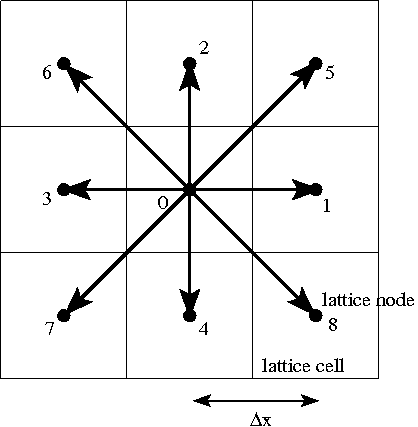
\includegraphics[width=0.3\linewidth]{D2Q9/D2Q9}
	\caption{Sketch of the D2Q9 lattice. Particles move exactly from a lattice node towards one of its nine neighbours (including the node itself) during one time step. By definition, the lattice spacing is related to the time step by $\Delta x/ \Delta t = \sqrt{3} c_s$ where $c_s$ is interpreted as a speed of sound.}
	\label{fig:D2Q9}
\end{figure}


% algo
%
The complexity of the flow emerges from the repeated application of simple rules of streaming and collision. The LB scheme advances the local densities of particles $f_i(\mathbf{x},t)$ moving with velocities $\mathbf{c}_i$  in a two-step procedure. Namely, an \emph{exact} streaming step 
\[
f_i(\mathbf{x}+\mathbf{c}_i \Delta t, t + \Delta t) = f_i^{\mathrm{out}}(\mathbf{x},t)
\]
during which particles move with their own velocity to a neighboring node, and an instantaneous collision step
\[
f_i^{\mathrm{out}}(\mathbf{x},t) = -\frac 1 {\tau_\nu} \left(f_i(\mathbf{x},t) - f_i^\mathrm{eq}(\mathbf{x},t) \right)
\]
which achieves a relaxation of local densities towards an absolute equilibrium (at the macroscopic level). The time-scale $\tau_\nu$ (in lattice unit) is related to the kinematic viscosity of the fluid by 
\[
\nu = \left( {\tau_\nu} - \frac 1 2 \right) c_s^2 ~\Delta t
\]
This simplification of the collision kernel is known as the BGK approximation in the kinetic theory of gas.
%
The equilibrium function is given  by
\[
f_i^\mathrm{eq}(\mathbf{x},t) = w_i  \rho(\mathbf{x},t) \left( 1 + \frac{\mathrm u(\mathbf{x},t) \cdot \mathbf{c_i}}{c_s^2} +
\frac{u_\alpha(\mathbf{x},t) u_\beta(\mathbf{x},t)({c_i}_\alpha {c_i}_\beta - c_s^2 \delta_{\alpha\beta})}{2 c_s^4} \right)
\] 
with the weight factors $w_0=4/9,~w_{1...4} = 1/9$ and $w_{5...8}=1/36$ for the D2Q9 lattice. Einstein summation convention is assumed.
Finally, let us mention that this discrete LB scheme is second-order accurate in $\Delta x $ and compliant to the weakly-compressible Navier-Stokes equations with a third-order error in $\mathrm{Ma}=|\mathbf{u}|/c_s$ as the lattice spacing vanishes, i.e. $\Delta x \to 0$. 

As mentioned before, the pressure is directly accessible from the mass density: $p = \rho c_s^2$. The viscous stress is also obtained easily from the densities of particles by
\[
\tau^\mathrm{visc.}_{\alpha \beta} = -\frac{\nu}{\tau_\nu ~ c_s^2 \Delta t} \sum_i  {c_i}_\alpha {c_i}_\beta (f_i - f_i^\mathrm{eq})
\]
so that the total stress expresses as
\begin{equation}\label{eq:def_stress}
\tau_{\alpha \beta} = -  c_s^2 \sum_i f_i ~ \delta_{\alpha\beta}  - \frac{\nu}{\tau_\nu ~ c_s^2 \Delta t} \sum_i  {c_i}_\alpha {c_i}_\beta (f_i - f_i^\mathrm{eq})
\end{equation}
Finally, let us mention that in the present context of turbulent flows, the single-relaxation-time BGK collision has been replaced by a multi-relaxation-time procedure based on central moments with an improved stability \cite{De_Rosis_2016}.

\bibliographystyle{unsrt}
\bibliography{biblio}

\end{document}
%%% Local Variables:
%%% mode: latex
%%% TeX-master: t
%%% End:
